\documentclass[11pt,onecolumn]{IEEEtran}
\usepackage{amsmath,amssymb,amsthm}
\usepackage{graphicx}
\usepackage{float}
\usepackage[hidelinks]{hyperref}

\newtheorem{theorem}{Theorem}
\newtheorem{proposition}[theorem]{Proposition}
\newtheorem{corollary}[theorem]{Corollary}
\newtheorem{lemma}[theorem]{Lemma}
\newtheorem{remark}[theorem]{Remark}

\newcommand{\E}{\mathbb{E}}
\newcommand{\R}{\mathbb{R}}
\newcommand{\C}{\mathbb{C}}
\newcommand{\tr}{\operatorname{tr}}
\newcommand{\Cov}{\operatorname{Cov}}
\newcommand{\hY}{\hat{\mathbf Y}}
\newcommand{\dw}{\tfrac{d\omega}{2\pi}}
\newcommand{\dl}{\tfrac{d\lambda}{2\pi}}
\newcommand{\herm}{\mathsf H}
\newcommand{\VG}{V_{\mathrm G}}
\newcommand{\RG}{\mathcal R_{\mathrm G}}
\newcommand{\tS}{\tilde\Sigma}
\newcommand{\cF}{\mathbb F}
\newcommand{\Vls}{V_{\mathrm{ls}}}
\newcommand{\op}{\mathrm{op}}
\newcommand{\fro}{\mathrm F}

\emergencystretch=1.5em
\begin{document}

\title{Rate, Leakage, and Distortion Beyond Stationary Gaussian Sources:\\ Water-Filling over Time and Frequency}

\author{Andrew~H.~Bond,~\IEEEmembership{Senior Member,~IEEE}%
\thanks{A. H. Bond is with the Department of Computer Engineering, San Jos\'e
State University, San Jos\'e, CA 95192 USA (e-mail: andrew.bond@sjsu.edu).
The manuscript sources and the check scripts of
Appendix~\ref{app:numver} are in the public repository named there.}}

\markboth{}{Bond: Rate, Leakage, and Distortion Beyond Stationary Gaussian Sources}

\maketitle

\begin{abstract}
An encoder describes part of a source to a decoder under a weighted
quadratic distortion. A second party holds a noisy observation of the
source and never decodes. The description has two costs, its rate and
its conditional leakage to the second party. The region of achievable
pairs is known for Gaussian vectors and for stationary Gaussian
processes, where it is water-filling on a tilted spectrum. Measured
signals are neither exactly stationary nor exactly Gaussian. We
determine the region for Gaussian sources whose covariance is locally
that of a stationary process with a spectrum that varies slowly in
time: it is water-filling over the time--frequency plane under one
water level. This holds for a fixed memoryless observation in white
noise, with deterministic encoders. For a cyclostationary source,
frequencies a multiple of the cycle frequency apart are coupled and
share one level. Averaging the spectrum over time never
lowers the cost. For a scalar Gaussian autoregressive source with
unstable poles, observed by the second party through a fixed nonzero
gain in white noise, each unstable pole costs the logarithm of its
modulus in rate and nothing in leakage. For a memoryless source that
is not Gaussian, the Gaussian region with the same second moments is
achievable, so the Gaussian source is the worst case for both costs.
Every code is bounded below by the Gaussian frontier less two
relative entropies, and this lower bound is asymptotically tight as
the distortion tends to zero when the whole source is reproduced.
\end{abstract}

\begin{IEEEkeywords}
Cyclostationary processes, equivocation, information leakage, locally
stationary processes, rate--distortion theory, secure source coding,
Shannon lower bound, water-filling.
\end{IEEEkeywords}

\section{Introduction}
\label{sec:intro}

An encoder observes a source and sends a description of part of it to
a decoder, which must reproduce that part within a weighted quadratic
distortion. A second party, the holder, has its own noisy observation
of the source. It sees the description but does not reconstruct
anything. The description costs its rate, and it costs what it tells
the holder beyond what the holder has, the conditional leakage. The
single-letter region of rate, distortion, and equivocation is due to
Villard and Piantanida \cite{villard2013}. For a Gaussian vector
source the frontier of rate against leakage was determined in
\cite{part1}: every frontier point is the fixed point of reverse
water-filling on the decoder's weight tilted by the holder's
information. For a stationary Gaussian process \cite{part2} proved that
the same holds frequency by frequency under one water level, and that
the resulting spectral region is the operational region.

\textbf{Why the stationary theory does not extend.} The proofs of
\cite{part2} use stationarity at every step. The Fourier transform
diagonalizes the source of period $n$. Window costs are subadditive
because every window has the same law. A window of a source with
finite memory is exactly a piece of a periodic source. And the coding
theorem separates a Gaussian process into a part of finite memory and
an independent remainder. For a source whose statistics change with
time there is no transform that diagonalizes it, windows have
different laws, and there is no periodic source to embed in. For a
source that is not Gaussian, uncorrelated parts are not independent
and the separation fails. The questions are also different. A source
that is not stationary has no spectral density, so one must first say
what replaces the spectral region. A source that is not Gaussian has
no closed-form region at all, and one asks for bounds. This paper
answers these questions with two tools that do not use stationarity
or a transform. The first compares the problem for a long Gaussian
vector with the problems for its blocks: the costs are superadditive
over blocks up to the information between the blocks, and a code for
a slightly smaller covariance serves a slightly larger one through a
coupling, whose randomness can be removed when the code is repeated on
many blocks with nearly the same law (Lemmas~\ref{lem:blocks},
\ref{lem:coupling}, and~\ref{lem:seeds}). The second
is a pair of maximum-entropy arguments for the two costs together
(Theorems~\ref{thm:inner} and~\ref{thm:outer}).

\textbf{Results for Gaussian sources that are not stationary.} The
main result is for a source whose covariance, on every short stretch
of time, is close to that of a stationary process with a local
spectral density $\Sigma(u,\omega)$ at the rescaled time $u\in[0,1]$.
This is local stationarity in the sense of Dahlhaus
\cite{dahlhaus1996}, stated through covariances. The operational
region is then given by reverse water-filling over the
time--frequency plane: the weighted cost is the minimum of
\[
\int_0^1\!\!\int_{-\pi}^{\pi}\bigl[\alpha r+(1-\alpha)\ell_{u,\omega}\bigr]\bigl(X(u,\omega)\bigr)\dw\,du
\]
over error spectra $X(u,\omega)$ that meet the distortion on average
over time and frequency, and the minimizer solves the tilted
water-filling equation of \cite{part2} at every time and frequency
with one common level (Theorem~\ref{thm:ls}). The theorem is an
operational statement about codes for the pair of costs, for a class
of sources given by their covariances. Its scope is narrower than that
of \cite{part2} in two ways, which we state here. The source must
satisfy three conditions on its covariances, (L1) to (L3) of
Section~\ref{sec:ls}, which describe a stable source that varies
slowly. And the holder observes each symbol through one fixed matrix in
white Gaussian noise, and the decoder's weight is fixed. As in
\cite{part1,part2}, deterministic encoders suffice. This needs a new
argument, because the removal of private randomness in \cite{part2}
repeats a code on windows that all have the same law
(Lemma~\ref{lem:seeds}). When the covariances and the local spectrum
are Lipschitz in time, no code of blocklength $N$, at a distortion
bounded away from zero, has a weighted cost more than a constant times
$N^{-1/2}$ below the frontier cost (Proposition~\ref{prop:rate}).
A source with more
power, or a holder with a better view, at one time than at another
draws rate at that time by the same rule that distributes rate over
frequency. With no holder, or at the weight that counts only the
rate, the theorem gives the rate--distortion function of a locally
stationary Gaussian vector process. We did not find that statement
for this class in the literature. The same lemmas give the region of
a source that becomes stationary: it is the spectral region of the
limit (Corollary~\ref{cor:as}). The stationary source with the
time-averaged spectrum has a region no larger: averaging the spectrum
over time never lowers the weighted cost at any weight
(Corollary~\ref{cor:lsavg}).

A cyclostationary source varies fast, with a period that does not
grow, and the block comparison does not apply. Its region is the
spectral region of the vector process obtained by stacking one period
(Theorem~\ref{thm:cyclo}). The stacking is the classical device of
Gladyshev \cite{gladyshev1961}, used for the rate--distortion function
by Kipnis, Goldsmith, and Eldar \cite{kipnis2018}, and the theorem is
a corollary of \cite{part2}. In the harmonic form of the stacked
spectrum (Proposition~\ref{prop:harmonic}) the frequencies split into
cosets of $q$ frequencies that differ by multiples of $2\pi/q$. Within
a coset the cyclic spectra couple the frequencies, and all cosets
share one water level. The stationary source with the time-averaged
spectrum again has a region no larger
(Theorem~\ref{thm:averaged}).

An autoregressive source with unstable poles varies neither slowly nor
periodically: its variance grows without bound, and (L3) excludes it.
For a scalar source of this kind with the memoryless holder, the region
is the spectral region of a stationary source moved by
$\sum\log|\rho_i|$ over the unstable poles $\rho_i$ in rate, and in
leakage only when the holder does not observe the source
(Theorem~\ref{thm:unstable}). At most as many eigenvalues of the
covariance as the order of the source are exceptional, and their
log-sum carries the growth. The holder sees those components with
bounded error, so their description costs rate but tells the holder
little. In this scalar model one allocation of the distortion is
optimal for both costs, and the region is a single quadrant
(Corollary~\ref{cor:quadrant}).

\textbf{Results for sources that are not Gaussian.} For a memoryless
source the Gaussian region with the same second moments is achievable
(Theorem~\ref{thm:inner}). The argument applies the Gaussian test
channel to the source as it is. That the rate is then no larger than
the Gaussian rate is classical. The leakage is a difference of two
mutual informations, and it is not obvious that it is controlled in
the same direction. It is, because with a Gaussian test channel the
leakage is a conditional entropy of the channel output less the
entropy of the channel noise, and only the first term depends on the
law of the source. Only second moments enter, so the holder's
observation need not be linear in the source. In the other direction,
every code is bounded below by the Gaussian frontier less a weighted
sum of two relative entropies, the distance of the source from the
Gaussian law with its covariance and the same distance conditionally
on the holder's observation (Theorem~\ref{thm:outer}). This is a
Shannon lower bound for the pair of costs. When the decoder reproduces
the whole source the lower bound is asymptotically tight as the
distortion tends to zero (Theorem~\ref{thm:highres}). The Gaussian
upper bound is then not attained, and the gap between the two bounds
stays equal to the weighted sum of the two relative entropies. Both bounds extend to stationary
processes, the lower bound for every process with a spectral density
and the upper bound for processes of finite dependence
(Theorems~\ref{thm:procouter} and~\ref{thm:procinner}).

The two halves of the paper meet in one place. The upper bound for
sources that are not Gaussian, applied to a mixture of Gaussian
sources, shows that the Gaussian frontier cost of an averaged
covariance is at least the cost of switching between the covariances
(Corollary~\ref{cor:mixing}). That statement about matrices is what
proves that averaging over time or over the phase of a cycle never
helps.

\textbf{Related work.} The rate--distortion function of a
cyclostationary Gaussian process was obtained by Kipnis, Goldsmith,
and Eldar \cite{kipnis2018} by stacking, and sampled cyclostationary
processes are treated in \cite{abakasanga2020}. For Gaussian vector
processes that are asymptotically stationary the rate--distortion
function is given in \cite{gutierrez2018}, by the asymptotic
equivalence of matrix sequences. Hammerich \cite{hammerich2016} proves
water-filling in the time--frequency plane for the rate--distortion
function of a class of nonstationary sources in continuous time, those
generated from white noise by a linear time-varying filter whose
symbol varies slowly. Theorem~\ref{thm:ls} is in discrete time, for
vector sources specified by their covariances, and has the second
party. The rate--distortion function of an unstable Gaussian
autoregressive source is due to Gray \cite{gray1970} and to Hashimoto
and Arimoto \cite{hashimoto1980}, whose two forms Gray and Hashimoto
\cite{grayhashimoto2008} showed to agree, and Tian and Kostina
\cite{tian2019} give coding theorems with second-order terms for the
first-order case. None of the works above has the second party. For sources that are not
Gaussian, the pattern of Theorems~\ref{thm:inner}
and~\ref{thm:outer}, variance in the upper bound and entropy power in
the lower, is that of the Shannon lower bound
\cite{berger1971,linder1994,koch2016} and of Lapidoth's result that
the Gaussian source is the hardest to describe at a given second
moment \cite{lapidoth1997}. Gastpar and Sula \cite{gastpar2024} give
bounds of this kind for conditional and Wyner--Ziv coding, and
Shomorony et al.\ \cite{shomorony2012} show that the Gaussian source is
the worst case for distributed quadratic coding. We found no bound of
either kind for the pair of rate and leakage, and no result with a
second party for sources that are not stationary. The search is
recorded in the repository named in Appendix~\ref{app:numver}. It was a
search of indexes and abstracts, and it is not proof of absence.

\section{Setting and Imported Results}
\label{sec:model}

Logarithms are base two unless written $\ln$, and entropies are in
bits. Norms of matrices are operator norms unless marked $\fro$ for
the Frobenius norm. Notation follows \cite{part1,part2}. In all three
papers the encoder observes the source $T$ and the decoder reproduces
the described part $Y=FT$, which is all of $T$ only when $F$ is
invertible.

\subsection{The memoryless problem}

The source emits independent copies $(T_i,S_i)$ of a pair $(T,S)$ with
$T\in\R^p$ centered, $\E\|T\|^2<\infty$, and covariance $K\succ0$. The
described variable is $Y=FT\in\R^m$ with $F$ of full row rank, the
decoder's weight is $W\succ0$, and $Q=F^{\mathsf T}WF$. The holder
observes $S\in\R^r$. A code of blocklength $n$ is an encoder
$f_n:\R^{p\times n}\to\mathcal M_n$, a finite set, and a decoder
$g_n:\mathcal M_n\to\R^{m\times n}$. With $M=f_n(T^n)$ and
$\hY^n=g_n(M)$,
\[
R_n=\tfrac1n\log|\mathcal M_n|,\quad
D_n=\tfrac1n\sum_{i=1}^n\E\bigl[(Y_i-\hY_i)^{\mathsf T}W(Y_i-\hY_i)\bigr],\quad
L_n=\tfrac1nH(M\mid S^n)=\tfrac1nI(T^n;M\mid S^n).
\]
A pair $(R,L)$ is achievable at distortion $D$ when codes of
blocklengths tending to infinity have $\limsup R_n\le R$,
$\limsup L_n\le L$, and $\limsup D_n\le D$.

The Gaussian problem of \cite{part1} is the case in which $T$ is
Gaussian and $S=HT+U$ with $U\sim\mathcal N(0,\Sigma_U)$ independent of
$T$ and $\Sigma_U\succ0$. Write $J=H^{\mathsf T}\Sigma_U^{-1}H$ and, for a
symmetric matrix $\Delta\succ0$,
\[
g(\Delta)=(\Delta^{-1}+J)^{-1}=\Delta-\Delta H^{\mathsf T}\bigl(H\Delta H^{\mathsf T}+\Sigma_U\bigr)^{-1}H\Delta ,
\]
the error covariance of the best linear estimate of a vector of
covariance $\Delta$ from its observation through $H$ in uncorrelated
noise of covariance $\Sigma_U$. For $0\prec\Delta\preceq K$ let
\begin{equation}
r(\Delta)=\tfrac12\log\frac{\det K}{\det\Delta},\qquad
\ell(\Delta)=\tfrac12\log\frac{\det g(K)}{\det g(\Delta)},
\label{eq:costs}
\end{equation}
and $\mathcal P(D)=\{\Delta:\ 0\prec\Delta\preceq K,\ \tr(Q\Delta)\le D\}$.
By \cite[Proposition~2 and Theorem~3]{part1} the closure of the
achievable set of the Gaussian problem is the union over
$\Delta\in\mathcal P(D)$ of the quadrants above
$(r(\Delta),\ell(\Delta))$, for $0<D<D_{\max}=\tr(QK)$. Both costs are
convex in $\Delta$ \cite[Theorem~5]{part1}. For $\alpha\in[0,1]$ let
\[
\VG(\alpha,D)=\min\bigl\{\alpha r(\Delta)+(1-\alpha)\ell(\Delta):\ \Delta\in\mathcal P(D)\bigr\},
\]
with $\VG(\alpha,D)=0$ for $D\ge D_{\max}$, and let $\RG(D)$ be the set
of pairs $(R,L)$ with $\alpha R+(1-\alpha)L\ge\VG(\alpha,D)$ for every
$\alpha\in[0,1]$, which is the region just described. The function
$\VG(\alpha,\cdot)$ is convex and nonincreasing. It depends on the data
only through $(K,Q,J)$, and we write $\VG(\alpha,D;K)$ when the
covariance varies.

For a pair $(T,S)$ that is not Gaussian, with $\E\|S\|^2<\infty$, the
Gaussian problem with the same second moments has
\begin{equation}
H=\Cov(S,T)K^{-1},\qquad\Sigma_U=\Cov(S)-\Cov(S,T)K^{-1}\Cov(T,S),
\label{eq:moments}
\end{equation}
and we assume $\Sigma_U\succ0$. If $S=HT+U$ with $U$ independent of $T$,
these are the matrix $H$ and the covariance of $U$.

\subsection{Gaussian vectors of several symbols}

Let $T=(T_1,\dots,T_n)\in\R^{pn}$ be a centered Gaussian vector with
covariance $\mathsf S\succ0$, and let the holder observe
$S_t=HT_t+U_t$ with $U_t$ independent $\mathcal N(0,\Sigma_U)$ and
independent of $T$, a memoryless map with white noise. A code for the
vector has an encoder that maps $T$, and private randomness
independent of $T$ and of the noise, to a message $M$ in a finite set,
and a decoder that maps $M$ to reproductions of $Y_t=FT_t$. Its rate,
distortion, and leakage per symbol are $\tfrac1n\log|\mathcal M|$,
$\tfrac1n\sum_t\E\|Y_t-\hY_t\|_W^2$, and $\tfrac1nH(M\mid S^n)$. The
frontier cost per symbol is
\[
\mathsf V_{\mathsf S}(\alpha,D)=\tfrac1n\VG\bigl(\alpha,D;\mathsf S\bigr)
\]
for the weight $\tfrac1nI_n\otimes Q$ and the holder
$(I_n\otimes H,I_n\otimes\Sigma_U)$. This is the quantity $V_S$ defined
before \cite[Lemma~11]{part2}. By \cite[Proposition~2]{part1}, every code for
the vector has $\alpha R+(1-\alpha)L\ge\mathsf V_{\mathsf S}(\alpha,D)$,
and the same holds for the pair $\tfrac1n(I(T;\Lambda),I(T;\Lambda\mid S^n))$
of any random variable $\Lambda$ with $\Lambda-T-S^n$ from which the
reproductions are computed. We use the order of the problem in the
covariance \cite[Lemma~11(b)]{part2}: if
$\mathsf S'\preceq\mathsf S\preceq(1+\kappa)\mathsf S'$, then for every
$D>0$
\begin{equation}
\mathsf V_{\mathsf S'}\bigl(\alpha,\tfrac{D}{1+\kappa}\bigr)-\tfrac p2\log(1+\kappa)\ \le\ \mathsf V_{\mathsf S}(\alpha,D)\ \le\ \mathsf V_{\mathsf S'}(\alpha,D)+\tfrac p2\log(1+\kappa).
\label{eq:order}
\end{equation}

\subsection{The stationary problem}

In \cite{part2} the source is a centered stationary Gaussian process
$(T_t)$ in $\R^p$ with a continuous positive definite spectral density
$\Sigma(\omega)$, the holder observes $S_t=\sum_kH_kT_{t-k}+U_t$ with a
continuous frequency response $H(\omega)$ and stationary Gaussian noise
of continuous positive definite spectral density $\Sigma_U(\omega)$, and
a code of blocklength $N$ acts on the window $T^N=(T_1,\dots,T_N)$,
with leakage $L_N=\tfrac1NH(M\mid S^N)$. For a Hermitian matrix
$0\prec X\preceq I$ the per-frequency rate, leakage, and distortion are
$r(X)=-\tfrac12\log\det X$, $\ell_\omega(X)$, and
$\tr(\tilde Q(\omega)X)$ with
$\tilde Q=\Sigma^{1/2}Q\Sigma^{1/2}$ \cite[Sec.~II]{part2}. The spectral
cost $V(\alpha,D)$ is the minimum of
$\int[\alpha r+(1-\alpha)\ell_\omega](X(\omega))\,\dw$ over fields with
$\int\tr(\tilde QX)\,\dw\le D$, the spectral region $\mathcal R(D)$ is
the set of pairs with $\alpha R+(1-\alpha)L\ge V(\alpha,D)$ for every
$\alpha$, and $D_{\max}=\int\tr(Q\Sigma)\,\dw$. The function
$V(\alpha,\cdot)$ is convex, nonincreasing, continuous, and zero from
$D_{\max}$ on. We use the following.
\begin{itemize}
\item[(i)] The closure $\mathcal A(D)$ of the achievable set equals
$\mathcal R(D)$ for $0<D<D_{\max}$, with deterministic encoders
\cite[Theorem~22]{part2}, and it is unchanged when the holder has its
observations on any set of times that contains the window
\cite[Theorem~23]{part2}. For a memoryless holder map and white noise
this is \cite[Theorem~16]{part2}, and by the third remark after that
theorem the codes exist at every large blocklength.
\item[(ii)] For a memoryless holder map $S_t=HT_t+U_t$ and white noise,
the window cost $V^{\mathrm w}_N$ is $\mathsf V_{\mathsf S}$ for the
covariance of $T^N$. It satisfies $V^{\mathrm w}_N\ge V$ for every
$D>0$, both being zero from $D_{\max}$ on, and
$V^{\mathrm w}_N\to V$ for $0<D<D_{\max}$, and every code of blocklength
$N$, with or without private randomness, has
$\alpha R_N+(1-\alpha)L_N\ge V(\alpha,D_N)$
\cite[Theorem~15]{part2}.
\item[(iii)] The cost per symbol $V_n(\alpha,D)$ of the source of period
$n$, whose covariance is the block-circulant matrix with the spectrum
sampled at the $n$ Fourier frequencies, converges to $V(\alpha,D)$ for
$0<D<D_{\max}$ \cite[Theorem~4]{part2}.
\item[(iv)] If $\Sigma'\preceq\Sigma\preceq(1+\kappa)\Sigma'$ at every
frequency, the inequalities \eqref{eq:order} hold for the spectral
costs \cite[Lemma~11(c)]{part2}.
\item[(v)] Let $K$ be a compact metric space carrying continuous data
$(\tilde Q,\tilde H,\Sigma_U)$ of a fixed size, and for a probability
measure $\mu$ on $K$ let $V_\mu(\alpha,D)$ be the minimum of
$\int[\alpha r+(1-\alpha)\ell_u](X(u))\,d\mu$ over fields with
$\int\tr(\tilde QX)\,d\mu\le D$. The minimum is attained by the field
that solves the tilted water-filling equation at every point with one
common level, and $V_{\mu_n}\to V_\mu$ when $\mu_n\to\mu$ weakly, for
$0<D<\int\tr\tilde Q\,d\mu$ \cite[Lemma~2]{part2}.
\end{itemize}
Theorem numbers of \cite{part1} are those of its submitted version,
and those of \cite{part2} are those of the version fixed by the tag
named in the references. They will be updated if either is revised.

\section{Memoryless Sources That Are Not Gaussian}
\label{sec:nongauss}

For a pair $(T,S)$ as in Section~\ref{sec:model} and $D>0$, call a
channel $p(\hat y\mid t)$ admissible at $D$ when its distortion
$\E\|Y-\hY\|_W^2$ is at most $D$. Information quantities of a channel
are computed under $p(t,s)p(\hat y\mid t)$, so that $\hY-T-S$ is a
Markov chain. Let
\[
V(\alpha,D)=\inf\bigl\{\alpha I(T;\hY)+(1-\alpha)I(T;\hY\mid S)\bigr\}
\]
over channels admissible at $D$. Both informations are convex in the
channel, so $V(\alpha,\cdot)$ is convex and nonincreasing. It is
finite for every $D>0$, because a quantizer of $T$ with finitely many
cells is admissible at $D$ when the cells are fine enough, by
$\E\|T\|^2<\infty$. Hence it is continuous on $(0,\infty)$.

\begin{proposition}\label{prop:coding}
Let $\E\|T\|^2<\infty$, $K\succ0$, and $I(T;S)<\infty$.
\begin{enumerate}
\item[(a)] For every code of blocklength $n$ there is a channel
admissible at $D_n$ with $I(T;\hY)\le R_n$ and
$I(T;\hY\mid S)\le L_n$. If $S=HT+U$ with $U$ independent of $T$, the
channel can be taken of the form $\hY=\phi(T,Z)$ with $Z$ independent
of $(T,U)$.
\item[(b)] For every channel admissible at $D$ with $I(T;\hY)<\infty$
and every $\epsilon>0$ there are, for every large $n$, deterministic
codes with $R_n\le I(T;\hY)+\epsilon$,
$L_n\le I(T;\hY\mid S)+\epsilon$, and $D_n\le D+\epsilon$.
\end{enumerate}
Consequently every achievable pair at $D$ satisfies
$\alpha R+(1-\alpha)L\ge V(\alpha,D)$ for every $\alpha$, and for every
$\alpha$ some achievable pair at $D$ has
$\alpha R+(1-\alpha)L\le V(\alpha,D)$.
\end{proposition}

\begin{proof}
This is the proof of \cite[Theorem~3]{part1} in its Appendix. That
proof uses the Gaussian law, or the additive form of the holder's
observation, at three points, and at a closedness step that is not
needed for the present statement.

(a) The converse there is the chain
$nR_n\ge I(T^n;\hY^n)\ge\sum_iI(T_i;\hY_i)$ and
\[
nL_n\ge I(T^n;\hY^n\mid S^n)=\sum_i\bigl[I(T_i;\hY^n,T^{i-1},S^n)-I(T_i;S_i)\bigr]\ge\sum_iI(T_i;\hY_i\mid S_i),
\]
which holds for independent identically distributed pairs with
$I(T;S)<\infty$. There the finiteness came from a Gaussian formula.
With $\tau$ uniform on $\{1,\dots,n\}$ and independent
of everything else, the channel from $T=T_\tau$ to $\hY=\hY_\tau$ has
the stated properties, because $(\tau,\hY)-T-S$ is a Markov chain: each
$\hY_i$ is a function of $T^n$, and given $T_i$ the observation $S_i$
is independent of the other letters. There this came from the
independence of the additive noise. In the additive case $\hY_\tau$ is
a function of $T_\tau$ and of $Z=(\tau,(T_i)_{i\ne\tau})$, and $U_\tau$
is independent of $(T^n,\tau)$.

(b) The achievability there quantizes $S$, $T$, and $\hY$ by nested
dyadic quantizers and applies the theorem of Villard and Piantanida
\cite{villard2013} to the quantized source. Positive definiteness of
the Gaussian covariance is used once, to say that every cell of the
quantizer of $T$ has positive probability. For a general law the cells
of probability zero are removed from the alphabet of the surrogate
source. The surrogate distortion
$\E[\|Y-\hat y\|_W^2\mid q_k(T)=t_k]$ is bounded for each level $k$
because the remaining cells are finitely many and $\E\|T\|^2<\infty$.
The convergence steps use martingale convergence, the Markov chain
$\hY-T-S$, and $\E\|\hY\|^2<\infty$, which follows from the finite
distortion. None uses the form of the law.

For the last statement, the first half follows from (a) and the
continuity of $V(\alpha,\cdot)$. For the second, take channels
admissible at $D$ with finite rate whose cost tends to $V(\alpha,D)$,
and codes from (b) with $\epsilon\to0$. Their pairs are bounded: the
leakage of a deterministic code is at most its rate, and since
$\hY-T-S$ is a Markov chain,
$I(T;\hY)=I(S;\hY)+I(T;\hY\mid S)\le I(T;S)+I(T;\hY\mid S)$, so the rates
are bounded when the costs are, also at $\alpha=0$. A limit point of
the pairs is achievable at $D$.
\end{proof}

\subsection{The Gaussian region is achievable}

\begin{theorem}\label{thm:inner}
Let $\E\|T\|^2<\infty$, $\E\|S\|^2<\infty$, $K\succ0$, and
$\Sigma_U\succ0$ in \eqref{eq:moments}. For every $D>0$ and every
$\Delta\in\mathcal P(D)$ there is a channel, with output $Z$ and a
reproduction that is a linear function of $Z$, with distortion
$\tr(Q\Delta)$ and
\[
I(T;Z)\le r(\Delta),\qquad I(T;Z\mid S)\le\ell(\Delta),
\]
where $r$ and $\ell$ are the costs \eqref{eq:costs} of the Gaussian
problem with the same second moments. Hence
$V(\alpha,D)\le\VG(\alpha,D)$ for every $\alpha$ and $D$, and if
$I(T;S)<\infty$ every pair of $\RG(D)$ is achievable for the source
$(T,S)$, for $0<D<D_{\max}$.
\end{theorem}

\begin{proof}
Factor $\Delta^{-1}-K^{-1}=G^{\mathsf T}G$ and let $Z=GT+N$ with
$N\sim\mathcal N(0,I_p)$ independent of $(T,S)$. The best linear
estimate of $T$ from $Z$ has error covariance
$(K^{-1}+G^{\mathsf T}G)^{-1}=\Delta$, so reproducing $Y$ by $F$ times
that estimate gives distortion $\tr(Q\Delta)$. The chain $Z-T-S$ holds.

For the rate, $I(T;Z)=h(Z)-h(N)$, and $h(Z)$ is at most the entropy of
the Gaussian vector with covariance $GKG^{\mathsf T}+I$. So
$I(T;Z)\le\tfrac12\log\det(I+GKG^{\mathsf T})=\tfrac12\log\det(K\Delta^{-1})=r(\Delta)$.

For the leakage, $h(Z\mid T,S)=h(N)$ because $N$ is independent of
$(T,S)$, so $I(T;Z\mid S)=h(Z\mid S)-h(N)$. For every matrix $B$,
$h(Z\mid S)\le h(Z-BS)$, which is at most the entropy of the Gaussian
vector with the covariance of $Z-BS$. Take $B$ to be the regression
matrix of $Z$ on $S$. By \eqref{eq:moments}, $\Cov(T,S)=KH^{\mathsf T}$
and $\Cov(S)=HKH^{\mathsf T}+\Sigma_U$, so the covariance of $Z-BS$ is
$Gg(K)G^{\mathsf T}+I$. Hence
\[
I(T;Z\mid S)\le\tfrac12\log\det\bigl(I+Gg(K)G^{\mathsf T}\bigr)
=\tfrac12\log\det\Bigl(g(K)\bigl(g(K)^{-1}+\Delta^{-1}-K^{-1}\bigr)\Bigr)
=\tfrac12\log\frac{\det g(K)}{\det g(\Delta)},
\]
since $g(K)^{-1}-K^{-1}=J$ and $\Delta^{-1}+J=g(\Delta)^{-1}$. The
reproduction is a function of $Z$, so its rate and leakage are no
larger. Minimizing over $\Delta$ gives $V\le\VG$, and
Proposition~\ref{prop:coding}(b) gives codes for every point
$(r(\Delta),\ell(\Delta))$, hence for $\RG(D)$.
\end{proof}

Three remarks. First, the theorem needs second moments only. The
holder's observation may be a nonlinear function of the source, or
have noise that depends on the source. The matrices $H$ and $\Sigma_U$
are then those of the best linear description of $S$ by $T$. Second,
the inequality for the rate is strict unless $Z$ is Gaussian, and the
one for the leakage is strict unless the residual $Z-BS$ is Gaussian
and independent of $S$. Third, the leakage of a general description
is a difference, $I(T;\hY)-I(S;\hY)$, and Gaussian data make the first
term largest for a Gaussian test channel but make the second term
largest too. The proof does not bound the two terms separately. It
writes the leakage as $h(Z\mid S)-h(N)$, in which only one term depends
on the law of the source.

\subsection{A lower bound for every code}

Suppose now that $S=HT+U$ with $U$ independent of $T$, of covariance
$\Sigma_U\succ0$ and of any law, that $T$ has a density with
$h(T)>-\infty$, and that $I(T;S)<\infty$. Let
$h(T\mid S)=h(T)-I(T;S)$ and
\begin{equation}
\vartheta(T)=\tfrac12\log\bigl((2\pi e)^p\det K\bigr)-h(T),\qquad
\vartheta(T\mid S)=\tfrac12\log\bigl((2\pi e)^p\det g(K)\bigr)-h(T\mid S).
\label{eq:deficits}
\end{equation}
The first is the relative entropy of the law of $T$ from the Gaussian
law with its covariance. The second is the same deficit for the
conditional law given the holder's observation. Both are nonnegative,
the second because the conditional entropy is at most that of the
error of the best linear estimate. When $U$ is Gaussian,
$\vartheta(T\mid S)=\vartheta(T)-\vartheta(S)\le\vartheta(T)$, because
then $I(T;S)=h(S)-h(U)$ and the Gaussian value of that information is
$\tfrac12\log((2\pi e)^r\det\Cov S)-h(U)$.

\begin{theorem}\label{thm:outer}
Under the assumptions of this subsection, let $\Lambda$ be a random
variable with values in a standard Borel space, with $(T,\Lambda)$
independent of $U$ and $I(T;\Lambda)<\infty$, and let
$\Delta=\E\Cov(T\mid\Lambda)$. Then $0\prec\Delta\preceq K$,
\begin{equation}
I(T;\Lambda)\ge r(\Delta)-\vartheta(T),\qquad
I(T;\Lambda\mid S)\ge\ell(\Delta)-\vartheta(T\mid S),
\label{eq:outer}
\end{equation}
and every reproduction of $Y$ that is a function of $\Lambda$ has
distortion at least $\tr(Q\Delta)$. Consequently, for every $\alpha$
and $D$,
\[
\VG(\alpha,D)-\alpha\vartheta(T)-(1-\alpha)\vartheta(T\mid S)\ \le\ V(\alpha,D)\ \le\ \VG(\alpha,D),
\]
and every code of blocklength $n$ satisfies
$\alpha R_n+(1-\alpha)L_n\ge\VG(\alpha,D_n)-\alpha\vartheta(T)-(1-\alpha)\vartheta(T\mid S)$.
\end{theorem}

\begin{proof}
Since $I(T;\Lambda)<\infty$, for almost every value $\lambda$ the
conditional law of $T$ has a density, so
$\Delta_\lambda=\Cov(T\mid\Lambda=\lambda)\succ0$ and $\Delta\succ0$, and
$\Delta\preceq K$ by the law of total covariance. The distortion of a
reproduction that is a function of $\Lambda$ is at least that of the
conditional mean, which is $\tr(Q\Delta)$.

For the rate, $I(T;\Lambda)=h(T)-h(T\mid\Lambda)$ and
$h(T\mid\Lambda=\lambda)\le\tfrac12\log((2\pi e)^p\det\Delta_\lambda)$. The
function $\log\det$ is concave, so averaging gives
$h(T\mid\Lambda)\le\tfrac12\log((2\pi e)^p\det\Delta)$. With the
definition of $\vartheta(T)$ this is the first inequality.

For the leakage, $\Lambda-T-S$ is a Markov chain because $U$ is
independent of $(T,\Lambda)$, so
$I(T;\Lambda,S)=I(T;\Lambda)+I(T;S)-I(\Lambda;S)$ is finite, and
$I(T;\Lambda\mid S)=h(T\mid S)-h(T\mid\Lambda,S)$. Fix $\lambda$. Under
the conditional law given $\Lambda=\lambda$, the noise $U$ is
independent of $T$ and has covariance $\Sigma_U$. So the best affine
estimate of $T$ from $S$ under that law has error covariance
$g(\Delta_\lambda)$, and
\[
h(T\mid S,\Lambda=\lambda)\le\tfrac12\log\bigl((2\pi e)^p\det g(\Delta_\lambda)\bigr).
\]
The map $g$ is concave in the L\"owner order. Indeed for every matrix
$B$ the error covariance of the estimate $BS$ is
$e_B(\Delta)=(I-BH)\Delta(I-BH)^{\mathsf T}+B\Sigma_UB^{\mathsf T}$, which
is affine in $\Delta$, and $g(\Delta)\preceq e_B(\Delta)$ with equality
for the best $B$. Taking $B$ best for $\Delta$,
$\E g(\Delta_\Lambda)\preceq\E e_B(\Delta_\Lambda)=e_B(\Delta)=g(\Delta)$.
Since $\log\det$ is concave and increasing,
$h(T\mid\Lambda,S)\le\tfrac12\log((2\pi e)^p\det g(\Delta))$. With the
definition of $\vartheta(T\mid S)$ this is the second inequality.

For the consequences, consider a channel admissible at $D$ with finite
weighted cost. Its leakage is finite when $\alpha<1$ and its rate when
$\alpha>0$, and by the Markov chain
$I(T;\hY)\le I(T;S)+I(T;\hY\mid S)$, so its rate is finite in every
case. A channel with output in $\R^m$ has the form $\hY=\phi(T,Z)$ in
law, with $Z$ independent of $(T,U)$. With $\Lambda=\hY$ it has
$\Delta\in\mathcal P(D)$, so its weighted cost is at least
$\alpha r(\Delta)+(1-\alpha)\ell(\Delta)-\alpha\vartheta(T)-(1-\alpha)\vartheta(T\mid S)$,
and $\alpha r(\Delta)+(1-\alpha)\ell(\Delta)\ge\VG(\alpha,D)$. The upper
bound is Theorem~\ref{thm:inner}. The statement for codes follows from
Proposition~\ref{prop:coding}(a).
\end{proof}

The lower bound is a Shannon lower bound for the pair of costs. At
$\alpha=1$ it reads $R(D)\ge R_{\mathrm G}(D)-\vartheta(T)$, which is the
classical bound in the range of $D$ where all components are
described \cite{berger1971}. For Gaussian holder noise the pair of
bounds says that the region of the source lies between the Gaussian
region and its translate by $\vartheta(T)$ bits in each coordinate.

\subsection{The lower bound is tight at high resolution}

\begin{lemma}\label{lem:entropy}
Let $X$ have a density on $\R^p$, $\E\|X\|^2<\infty$, and
$h(X)>-\infty$, and let $N_j\sim\mathcal N(0,\Gamma_j)$ be independent
of $X$ with $\Gamma_j\to0$. Then $h(X+N_j)\to h(X)$. If moreover $X$ is
jointly distributed with $S$, $N_j$ is independent of $(X,S)$, and
$I(X;S)<\infty$, then $h(X+N_j\mid S)\to h(X\mid S)$.
\end{lemma}

\begin{proof}
$h(X+N_j)\ge h(X+N_j\mid N_j)=h(X)$. For the other direction let
$\gamma$ be the standard Gaussian density on $\R^p$. In nats, for a
law $P$ with a density and finite second moment,
$h(P)=-D(P\|\gamma)+\tfrac p2\ln2\pi+\tfrac12\E_P\|X\|^2$. The laws of
$X+N_j$ converge weakly to that of $X$ and their second moments
converge. Relative entropy is lower semicontinuous under weak
convergence, being a supremum of weakly continuous functionals
\cite{gray1990eit}. So $\limsup h(X+N_j)\le h(X)$.

For the conditional statement, for almost every $s$ the conditional
law of $X$ given $S=s$ has a density and a finite second moment, and
the first part gives $h(X+N_j\mid S=s)\to h(X\mid S=s)$, also when the
right side is $-\infty$. Moreover
\[
h(X\mid S=s)\le h(X+N_j\mid S=s)\le\tfrac p2\log\Bigl(\tfrac{2\pi e}{p}\bigl(\tr\Cov(X\mid S=s)+\tr\Gamma_j\bigr)\Bigr).
\]
The right side is bounded by an affine function of
$\tr\Cov(X\mid S=s)$, which is integrable, and the left side is
integrable because its integral $h(X)-I(X;S)$ is finite and it is
bounded above by an integrable function. Dominated convergence gives
the claim.
\end{proof}

\begin{theorem}\label{thm:highres}
Under the assumptions of Theorem~\ref{thm:outer}, suppose $Q\succ0$.
Then for every $\alpha\in[0,1]$, as $D\to0$,
\[
V(\alpha,D)-\bigl[\VG(\alpha,D)-\alpha\vartheta(T)-(1-\alpha)\vartheta(T\mid S)\bigr]\ \to\ 0 .
\]
\end{theorem}

\begin{proof}
The difference is nonnegative by Theorem~\ref{thm:outer}. Let
$\Delta$ be a minimizer of $\VG(\alpha,D)$. Since $Q\succeq\underline qI$ for
some $\underline q>0$ and $\tr(Q\Delta)\le D$, we have
$\Delta\preceq(D/\underline q)I$, so for small $D$ the matrix
$\Delta^{-1}-K^{-1}$ is positive definite and
$\Gamma=(\Delta^{-1}-K^{-1})^{-1}\to0$ as $D\to0$. The channel of
Theorem~\ref{thm:inner} has $G$ invertible, and $G^{-1}Z=T+N'$ with
$N'\sim\mathcal N(0,\Gamma)$. From the proof of that theorem, its cost
is $\VG(\alpha,D)$ less
\[
\alpha\bigl[h_{\mathrm G}(Z)-h(Z)\bigr]+(1-\alpha)\bigl[h_{\mathrm G}(Z\mid S)-h(Z\mid S)\bigr],
\]
where $h_{\mathrm G}$ denotes the two Gaussian bounds used there. Both
brackets are unchanged by the invertible map $G^{-1}$. In terms of
$T+N'$ they are
$\tfrac12\log((2\pi e)^p\det(K+\Gamma))-h(T+N')$ and
$\tfrac12\log((2\pi e)^p\det(g(K)+\Gamma))-h(T+N'\mid S)$, because the
error of the best linear estimate of $T+N'$ from $S$ has covariance
$g(K)+\Gamma$. By Lemma~\ref{lem:entropy} they tend to $\vartheta(T)$ and
$\vartheta(T\mid S)$. So
$V(\alpha,D)\le\VG(\alpha,D)-\alpha\vartheta(T)-(1-\alpha)\vartheta(T\mid S)+o(1)$.
\end{proof}

So at high resolution the cost of the source is the Gaussian cost
less the weighted deficits, to within a vanishing term, and the
Gaussian test channel attains it. The upper bound $\VG$ of
Theorem~\ref{thm:inner} stays above it by
$\alpha\vartheta(T)+(1-\alpha)\vartheta(T\mid S)$.
When $Q$ is singular some directions of the source are never
described, however small the distortion, and the argument does not
apply to them. We do not know the limit in that case.

\subsection{Mixing covariances}

\begin{corollary}\label{cor:mixing}
Let $K_1,\dots,K_C\succ0$, let $\lambda_c>0$ sum to one, and let
$\bar K=\sum_c\lambda_cK_c$. For the Gaussian problems with a common
$(Q,H,\Sigma_U)$, every $\alpha\in[0,1]$, and every $D>0$,
\[
\VG(\alpha,D;\bar K)\ \ge\ \min\Bigl\{\sum_c\lambda_c\VG(\alpha,D_c;K_c):\ \sum_c\lambda_cD_c\le D\Bigr\}.
\]
If $K_c=O_cKO_c^{\mathsf T}$ for orthogonal matrices $O_c$ with
$O_c^{\mathsf T}QO_c=Q$ and $O_c^{\mathsf T}JO_c=J$, then
$\VG(\alpha,D;\bar K)\ge\VG(\alpha,D;K)$.
\end{corollary}

\begin{proof}
Let $\Theta$ take the value $c$ with probability $\lambda_c$, let $T$
be Gaussian with covariance $K_\Theta$ given $\Theta$, and let
$S=HT+U$ with $U\sim\mathcal N(0,\Sigma_U)$ independent of
$(T,\Theta)$. Then $T$ has covariance $\bar K$, and the Gaussian
problem with the same second moments is that of $\bar K$. Let
$\Delta$ attain $\VG(\alpha,D;\bar K)$, for $D<\tr(Q\bar K)$, and let
$Z$ be the channel of Theorem~\ref{thm:inner}, so that
$\alpha I(T;Z)+(1-\alpha)I(T;Z\mid S)\le\VG(\alpha,D;\bar K)$. Since
$\Theta-T-(Z,S)$ is a Markov chain,
\[
I(T;Z)=I(\Theta;Z)+I(T;Z\mid\Theta)\ge I(T;Z\mid\Theta),\qquad
I(T;Z\mid S)=I(\Theta;Z\mid S)+I(T;Z\mid S,\Theta)\ge I(T;Z\mid S,\Theta).
\]
Given $\Theta=c$ the source is Gaussian with covariance $K_c$ and the
channel with its linear reproduction is admissible at its distortion
$D_c$ under that law, with $\sum_c\lambda_cD_c=\tr(Q\Delta)\le D$. By
\cite[Proposition~2]{part1} its weighted cost given $\Theta=c$ is at
least $\VG(\alpha,D_c;K_c)$. This gives the first statement. For
$D\ge\tr(Q\bar K)$ the right side is zero, with $D_c=\tr(QK_c)$. For
the second, the substitution $\Delta\mapsto O_c\Delta O_c^{\mathsf T}$
maps the program of $K$ onto that of $K_c$ and preserves the costs and
the distortion, so $\VG(\cdot,\cdot;K_c)=\VG(\cdot,\cdot;K)$, and
$\sum_c\lambda_c\VG(\alpha,D_c;K)\ge\VG(\alpha,D;K)$ by convexity and
monotonicity in the distortion.
\end{proof}

The corollary is a statement about matrices, and its proof passes
through a source that is not Gaussian. A Gaussian source whose
covariance is an average costs at least as much as a source that
switches between the covariances, at every weight. For $\alpha=1$ this
is the familiar fact that a Gaussian source is harder to describe than
any other source with its covariance, applied to a mixture.

\section{Stationary Processes That Are Not Gaussian}
\label{sec:procs}

Let $(T_t)_{t\in\mathbb Z}$ be a centered stationary process in $\R^p$
with finite second moments and a continuous positive definite
spectral density $\Sigma$. It need not be Gaussian. The holder observes
$S_t=HT_t+U_t$, where the $U_t$ are independent and identically
distributed, of covariance $\Sigma_U\succ0$ and any law, and
independent of the process $T$. Codes, their rate, distortion, and
leakage, and $\mathcal A(D)$ are as in \cite{part2}, with private
randomness at the encoder allowed and independent of both processes.
The spectral cost $V$ and the window costs $V^{\mathrm w}_N$ are those
of the Gaussian process with spectral density $\Sigma$ and the Gaussian
holder with the same $(H,\Sigma_U)$. Suppose that every window $T^N$ has
a density with $h(T^N)>-\infty$ and that $I(T^N;S^N)<\infty$. Let
$\vartheta_N=\vartheta(T^N)$ and
$\vartheta'_N=\vartheta(T^N\mid S^N)$ be the deficits
\eqref{eq:deficits} of the window, a vector in $\R^{pN}$ with the
block-Toeplitz covariance of the window and the holder
$(I_N\otimes H,I_N\otimes\Sigma_U)$.

\begin{theorem}\label{thm:procouter}
Every code of blocklength $N$ for the process satisfies, for every
$\alpha\in[0,1]$,
\[
\alpha R_N+(1-\alpha)L_N\ \ge\ V^{\mathrm w}_N(\alpha,D_N)-\frac{\alpha\vartheta_N+(1-\alpha)\vartheta'_N}{N}
\ \ge\ V(\alpha,D_N)-\frac{\alpha\vartheta_N+(1-\alpha)\vartheta'_N}{N}.
\]
The limit $\bar\vartheta=\lim\vartheta_N/N$ exists in $[0,\infty]$ and
equals
$\int\tfrac12\log\bigl((2\pi e)^p\det\Sigma(\omega)\bigr)\dw$ less the
entropy rate of the process. If the noise is Gaussian,
$\vartheta'_N\le\vartheta_N$, and every pair achievable at $D$
satisfies $\alpha R+(1-\alpha)L\ge V(\alpha,D)-\bar\vartheta$ for every
$\alpha$.
\end{theorem}

\begin{proof}
Apply Theorem~\ref{thm:outer} to the vector $T^N$, the holder
$(I_N\otimes H,U^N)$, the weight $\tfrac1NI_N\otimes Q$, and
$\Lambda=M$. The message is a function of $T^N$ and of private
randomness independent of both processes, so $(T^N,M)$ is independent
of $U^N$, and $I(T^N;M)\le\log|\mathcal M|$. Since
$NR_N\ge I(T^N;M)$ and $NL_N=H(M\mid S^N)\ge I(T^N;M\mid S^N)$, the
weighted cost of the code is at least
$\alpha r(\Delta)+(1-\alpha)\ell(\Delta)-\alpha\vartheta_N-(1-\alpha)\vartheta'_N$
for a matrix $\Delta$ feasible in the window problem at $D_N$, and the
first two terms are at least $N\,V^{\mathrm w}_N(\alpha,D_N)$. The second
inequality is item~(ii) of Section~\ref{sec:model}. The entropies
$h(T^N)/N$ converge to the entropy rate, a number in $[-\infty,\infty)$,
because $h(T_N\mid T^{N-1})$ is nonincreasing by stationarity, and
$\tfrac1N\log\det T_N(\Sigma)\to\int\log\det\Sigma\,\dw$ by the Szeg\H{o}
limit theorem for matrix symbols \cite[Lemma~14]{part2}. The last
statement follows from $\vartheta'_N\le\vartheta_N$ for Gaussian noise
and the continuity of $V(\alpha,\cdot)$. It is empty when the entropy
rate is $-\infty$.
\end{proof}

\begin{theorem}\label{thm:procinner}
Suppose in addition that the process has finite dependence: for some
$m$ and every $a$, $(T_t)_{t\le a}$ and $(T_t)_{t>a+m}$ are independent.
Then for $0<D<D_{\max}$ every pair of the spectral region
$\mathcal R(D)$ is achievable, with deterministic encoders.
\end{theorem}

\begin{proof}
Fix $0<\alpha<1$, $\delta>0$, and $n$. Divide $\{1,\dots,N\}$,
$N=k(n+m)$, into $k$ segments, each a block of $n$ symbols followed by
a guard interval of $m$ symbols. Blocks in different segments are
separated by more than $m$ symbols, so they are independent, and the
noise is independent across time. The pairs formed by a block and the
holder's observations in it are therefore independent and identically
distributed. They form a memoryless source with letters in $\R^{pn}$
whose letter has the covariance of the window, a finite second
moment, and $I(T^n;S^n)<\infty$. The Gaussian problem with the same
second moments is the window problem of size $n$. By
Theorem~\ref{thm:inner} and Proposition~\ref{prop:coding}(b), for the
frontier point of weight $\alpha$ of the window problem at $D$ there
are, for large $k$, deterministic codes on the $k$ blocks whose
weighted cost per symbol of the blocks is at most
$V^{\mathrm w}_n(\alpha,D)+\delta$ and whose distortion per symbol of the
blocks is at most $D+\delta$. Use such a code on the blocks and
reproduce zero in the guard intervals. The rate per symbol does not
increase. Conditioning on the holder's observations in the guard
intervals does not raise the entropy of the message, so the leakage
per symbol does not increase. The distortion is at most
$D+\delta+\tfrac m{n+m}D_{\max}$. As $n\to\infty$,
$V^{\mathrm w}_n(\alpha,D)\to V(\alpha,D)$ by item~(ii). So for every
$\delta$ there are deterministic codes of arbitrarily large blocklength
with $D_N\le D+2\delta$ and
$\alpha R_N+(1-\alpha)L_N\le V(\alpha,D)+2\delta$. Their pairs are
bounded, and a limit point is achievable at $D$ by deterministic codes
with weighted cost at most $V(\alpha,D)$.

Let $\mathcal A_{\mathrm d}(D)$ be the closure of the set of pairs
achievable at $D$ by deterministic codes. It is closed, upward closed,
and contained in the nonnegative quadrant. It is convex by time
sharing: copies of two codes used on consecutive windows, in numbers
that give a rational weight exactly as in the proof of
\cite[Theorem~16]{part2}, have a rate and a distortion that are the
weighted averages, and a leakage at most the weighted average, by
\cite[Lemma~18]{part2}. The proof of that lemma uses only that the
source and the noise are stationary and independent of each other and
that the entropy of a tuple of messages is at most the sum of the
entropies, and the resulting encoder is deterministic when the given
ones are. A closed, convex, upward closed subset of the nonnegative
quadrant is the intersection of its supporting half-planes with
normals $(\alpha,1-\alpha)$, $0<\alpha<1$ \cite[proof of
Theorem~16]{part2}, and the support value of
$\mathcal A_{\mathrm d}(D)$ at each such normal is at most
$V(\alpha,D)$. So $\mathcal A_{\mathrm d}(D)\supseteq\mathcal R(D)$.
\end{proof}

For example, let $T_t=\sum_{j=0}^mB_jW_{t-j}$ with independent
identically distributed innovations $W_t$ in $\R^p$ that have a
density, a finite variance, and $h(W)>-\infty$, with $B_0$ invertible
and $\det\sum_jB_je^{-i\omega j}\ne0$ at every frequency. The process has
dependence $m$ and a continuous positive definite spectral density,
and $h(T^N)\ge h(T^N\mid W_{1-m},\dots,W_0)=N\,h(W)+N\log|\det B_0|$, so
both theorems apply. With Gaussian holder noise they place the
operational region between the spectral region and its translate by
the relative entropy rate $\bar\vartheta$. The upper bound is not
proved here for processes of infinite dependence. The decomposition
of \cite[Theorem~16]{part2} into a part of finite memory and a
remainder of small power uses the Gaussian law to make the two parts
independent.

\section{Gaussian Vectors: Blocks and Couplings}
\label{sec:tools}

This section has no stationarity in it. It compares the problem of
Section~\ref{sec:model} for a Gaussian vector of many symbols with the
problems for its blocks, in both directions. The three lemmas that
matter can be read as follows.
\begin{itemize}
\item Lemma~\ref{lem:blocks} is the converse tool. Cut a long vector
into blocks. Any code for the whole vector is, block by block, a
description of that block, and the costs add up, except that
correlation between the blocks lets one block's description serve
another. The lemma says that this saving is at most the mutual
information between the blocks, which Lemma~\ref{lem:cut} bounds by the
size of their cross-covariance. For a source whose past and future are
weakly correlated the saving stays bounded while the costs grow with
the length.
\item Lemma~\ref{lem:coupling} is the achievability tool. A vector with
a slightly larger covariance is the sum of a vector with the smaller
covariance and an independent small remainder. The encoder draws that
decomposition, describes the first part with a code made for it, and
ignores the remainder. The remainder adds its power to the distortion,
and it tells the holder little because it is small.
\item Lemma~\ref{lem:seeds} removes the randomness of that draw. One code
is repeated on many consecutive blocks whose covariances are all
slightly larger than the one it was made for. Each block gets a fixed
seed, and the seeds are chosen so that the averages over the blocks of
the distortion and of the leakage are close to their means.
\end{itemize}
The proofs use only the chain rule, maximum entropy for Gaussian
vectors, and \cite[Proposition~2]{part1}.

\begin{lemma}\label{lem:cut}
Let $X$ and $Y$ be jointly Gaussian vectors whose joint covariance has
all eigenvalues in $[a_0,b_0]$, $0<a_0\le b_0$, and let $C$ be their
cross-covariance. Then
$I(X;Y)\le\dfrac{b_0}{2a_0^3\ln2}\,\|C\|_{\fro}^2$.
\end{lemma}

\begin{proof}
Let $A$ and $B$ be the covariances of $X$ and $Y$ and
$\mathsf C=A^{-1/2}CB^{-1/2}$. In nats
$2I(X;Y)=-\ln\det(I-\mathsf C\mathsf C^{\mathsf T})$. The conditional
covariance $A-CB^{-1}C^{\mathsf T}$ is at least $a_0I$ and
$A\preceq b_0I$, so $I-\mathsf C\mathsf C^{\mathsf T}\succeq(a_0/b_0)I$. For
$0\le x\le1-a_0/b_0$, $-\ln(1-x)\le(b_0/a_0)x$. Hence
$2I\le(b_0/a_0)\tr(\mathsf C\mathsf C^{\mathsf T})\le(b_0/a_0^3)\|C\|_{\fro}^2$.
This is the estimate in the proof of \cite[Lemma~14]{part2}.
\end{proof}

\begin{lemma}\label{lem:blocks}
Let $T=(T_1,\dots,T_N)$ be a centered Gaussian vector in $\R^{pN}$ with
covariance $\mathsf S$, $a_0I\preceq\mathsf S\preceq b_0I$, with the
memoryless holder of Section~\ref{sec:model}. Split the times into
consecutive blocks $I_1,\dots,I_B$ of lengths $n_1,\dots,n_B$, and let
$\chi_b=\|\Cov(T_{I_1\cup\dots\cup I_{b-1}},T_{I_b})\|_{\fro}^2$. For
every code for the vector, with or without private randomness, with
distortion $D_b$ per symbol in block $b$, and every $\alpha\in[0,1]$,
\[
N\bigl[\alpha R+(1-\alpha)L\bigr]\ \ge\ \sum_{b=1}^Bn_b\,\mathsf V_{\mathsf S[I_b]}(\alpha,D_b)\ -\ c_1\sum_{b=2}^B\chi_b ,
\]
where $\mathsf S[I_b]$ is the covariance of block $b$ and
$c_1=b_0/(2a_0^3\ln2)$.
\end{lemma}

\begin{proof}
Write $T_b$ and $S_b$ for the source and the holder's observation in
block $b$, and $S$ for the whole observation. Since
$NR\ge I(T;M)$ and $NL=H(M\mid S)\ge I(T;M\mid S)$, it suffices to bound
the two informations.

\emph{Rate.}
$I(T;M)=h(T)-h(T\mid M)\ge h(T)-\sum_bh(T_b\mid M)=\sum_bI(T_b;M)-\mathsf c(T)$,
with $\mathsf c(T)=\sum_bh(T_b)-h(T)=\sum_{b\ge2}I(T_b;T_1,\dots,T_{b-1})$.

\emph{Leakage.} The message takes finitely many values, so all
entropies below are finite, and
\[
I(T;M\mid S)=h(T\mid S)-h(T\mid M,S)\ge h(T\mid S)-\sum_bh(T_b\mid M,S_b)
=\sum_bI(T_b;M\mid S_b)-\mathsf c(T\mid S),
\]
with $\mathsf c(T\mid S)=\sum_bh(T_b\mid S_b)-h(T\mid S)$. Since
$h(T_b\mid S_b)=h(T_b,S_b)-h(S_b)$ and $h(T\mid S)=h(T,S)-h(S)$,
\begin{align*}
\mathsf c(T\mid S)&=\Bigl[\sum_bh(T_b,S_b)-h(T,S)\Bigr]-\Bigl[\sum_bh(S_b)-h(S)\Bigr]\\
&\le\sum_{b\ge2}I\bigl(T_b,S_b;\,T_1,S_1,\dots,T_{b-1},S_{b-1}\bigr)
=\sum_{b\ge2}I\bigl(T_b;\,T_1,\dots,T_{b-1}\bigr)=\mathsf c(T),
\end{align*}
because the second bracket is nonnegative, and because each
observation is its own block of the source seen through a memoryless
map in independent noise, so that
$(S_1,\dots,S_{b-1})-(T_1,\dots,T_{b-1})-T_b-S_b$ is a Markov chain.

\emph{The blocks.} For each $b$, the message is a function of $T$ and
of private randomness independent of the noise, and $S_b$ is $T_b$
seen through a memoryless map in noise independent of everything
else. So $M-T_b-S_b$ is a Markov chain, and the reproduction of block
$b$ is a function of $M$ with distortion $D_b$ per symbol. By the
statement of Section~\ref{sec:model} for the Gaussian vector $T_b$,
$\alpha I(T_b;M)+(1-\alpha)I(T_b;M\mid S_b)\ge n_b\mathsf V_{\mathsf S[I_b]}(\alpha,D_b)$.

\emph{The cuts.} The covariance of $(T_1,\dots,T_b)$ is a principal
submatrix of $\mathsf S$, so its eigenvalues lie in $[a_0,b_0]$, and by
Lemma~\ref{lem:cut},
$I(T_b;T_1,\dots,T_{b-1})\le b_0\chi_b/(2a_0^3\ln2)$. So
$\mathsf c(T\mid S)\le\mathsf c(T)\le c_1\sum_{b\ge2}\chi_b$, and
$\alpha\mathsf c(T)+(1-\alpha)\mathsf c(T\mid S)$ is at most the same.
\end{proof}

For independent blocks the cut terms vanish and the lemma is the
counterpart for codes of the splitting of \cite[Theorem~12]{part1}. The
lemma says that dependence
between blocks can lower the weighted cost by at most the information
between them, for the rate and for the leakage alike.

\begin{lemma}\label{lem:coupling}
Let $0\prec\mathsf S'\preceq\mathsf S$ be covariances of Gaussian
vectors of $n$ symbols, with the memoryless holder of
Section~\ref{sec:model}.
Suppose a code for the vector with covariance $\mathsf S'$ has rate
$R'$, distortion $D'$, and leakage $L'$. Then there is a code for the
vector with covariance $\mathsf S$, with private randomness, with
\[
R=R',\qquad D\le D'+\tfrac1n\tr\bigl((I_n\otimes Q)(\mathsf S-\mathsf S')\bigr),\qquad
L\le L'+\tfrac1{2n\ln2}\tr\bigl((I_n\otimes J)(\mathsf S-\mathsf S')\bigr).
\]
\end{lemma}

\begin{proof}
This is the coupling in the proof of \cite[Theorem~16]{part2}, which
does not use stationarity. Given $T\sim\mathcal N(0,\mathsf S)$ the
encoder draws $T'$ from the conditional law of the first summand
given the sum, for independent $T'\sim\mathcal N(0,\mathsf S')$ and
$E\sim\mathcal N(0,\mathsf S-\mathsf S')$, and applies the given code to
$T'$. Then $T'$, $E=T-T'$, the noise $U$, and the private randomness
of the given code are independent. The holder sees
$S=S'+(I_n\otimes H)E$ with $S'=(I_n\otimes H)T'+U$, and $(T',S')$ has
the law for which the code was made. The reproduction is a function of
$T'$ and of randomness independent of $E$, and $E$ is centered, so
$\E\|Y_t-\hY_t\|_W^2=\E\|FT'_t-\hY_t\|_W^2+\E\|FE_t\|_W^2$, which gives
the distortion. For the leakage,
$H(M\mid S)=H(M\mid S,E)+I(M;E\mid S)$. Given $E$ the observations $S$
and $S'$ determine each other, and $(M,S')$ is independent of $E$, so
the first term is $H(M\mid S')=nL'$. For the second, let $Z'$ be the
private randomness of the given code, so that $M$ is a function of
$(T',Z')$, and $(T',Z')$ is independent of $(E,U)$. Then
$I(M;E\mid S)\le I(T',Z';E\mid S)\le I(E;T',Z',S)=I(E;S\mid T',Z')=I(E;(I_n\otimes H)E+U)$,
which is at most
$\tfrac1{2\ln2}\tr((I_n\otimes J)(\mathsf S-\mathsf S'))$ by
$\ln\det(I+C)\le\tr C$.
\end{proof}

The draw can be written with an explicit seed. With
$\mathsf A=\mathsf S'\mathsf S^{-1}$, a matrix $\mathsf C$ with
$\mathsf C\mathsf C^{\mathsf T}=\mathsf S'-\mathsf S'\mathsf S^{-1}\mathsf S'$,
which is positive semidefinite because $\mathsf S'\preceq\mathsf S$, and
a seed $\zeta\sim\mathcal N(0,I)$ independent of everything else, the
vector $T'=\mathsf AT+\mathsf C\zeta$ has covariance $\mathsf S'$ and is
uncorrelated with $T-T'$, so the pair has the law required in the
proof.

\begin{lemma}\label{lem:seeds}
Let a code with a deterministic encoder for the Gaussian vector of
$n_0$ symbols with covariance $\mathsf S'\succ0$ have rate $R'$,
distortion $D'$, and leakage $L'$. Let $T$ be a Gaussian vector of
$kn_0$ symbols, with the memoryless holder of Section~\ref{sec:model},
whose $k$ consecutive sub-vectors of $n_0$ symbols have covariances
$\mathsf S_1,\dots,\mathsf S_k$ with
$\mathsf S'\preceq\mathsf S_j\preceq b_0I$ and
\[
\tfrac1{n_0}\tr\bigl((I_{n_0}\otimes Q)(\mathsf S_j-\mathsf S')\bigr)\le\epsilon_Q,\qquad
\tfrac1{2n_0\ln2}\tr\bigl((I_{n_0}\otimes J)(\mathsf S_j-\mathsf S')\bigr)\le\epsilon_J .
\]
The sub-vectors may be dependent. For every $\delta>0$ there is $k_0$,
which depends only on the code, $b_0$, $Q$, and $\delta$, such that for
$k\ge k_0$ there is a code for $T$ with a deterministic encoder, rate
$R'$, distortion at most $D'+\epsilon_Q+\delta$, and leakage at most
$L'+\epsilon_J+\delta$.
\end{lemma}

\begin{proof}
For the $j$th sub-vector $T_j$ and a seed $z$ let
$T'_j=\mathsf A_jT_j+\mathsf C_jz$ be the draw above for
$\mathsf S_j$, let $M_j(z)$ be the message of the given code applied
to $T'_j$, and let $D_j(z)$ and $L_j(z)=\tfrac1{n_0}H(M_j(z)\mid S_j)$ be
the distortion and the leakage per symbol of the resulting
deterministic code for $T_j$, where $S_j$ is the holder's observation
of the sub-vector. Both are measurable in $z$ by Tonelli's theorem, as
in the proof of \cite[Lemma~19]{part2}, the encoder being a measurable
map. With a random seed
$\zeta\sim\mathcal N(0,I)$ this is the code of
Lemma~\ref{lem:coupling}, so
$\E D_j(\zeta)\le D'+\epsilon_Q$, and
$\E L_j(\zeta)=\tfrac1{n_0}H(M_j\mid S_j,\zeta)\le\tfrac1{n_0}H(M_j\mid S_j)\le L'+\epsilon_J$,
because conditioning on the seed does not raise the entropy.

The leakages $L_j(z)$ lie in $[0,R']$. For the distortions, the
reproductions of the given code take finitely many values, so their
norms $\|\cdot\|_W$ are at most some $\varrho$, and by Jensen's inequality
$\E D_j(\zeta)^2$ is at most the second moment of
$\tfrac1{n_0}\sum_t\|Y_t-\hY_t\|_W^2$, which is at most
$\tfrac1{n_0}\sum_t\E(2\|Y_t\|_W^2+2\varrho^2)^2\le24(b_0\tr Q)^2+8\varrho^4$,
since $\E\|Y_t\|_W^4\le3(\tr(Q\Cov T_t))^2$ for a Gaussian vector. Call
this bound $v$. It does not depend on $j$ or on $k$.

Take independent seeds $\zeta_1,\dots,\zeta_k$. The variables
$D_j(\zeta_j)$ are independent with variances at most $v$, and the
variables $L_j(\zeta_j)$ are independent with variances at most
$R'^2$. By Chebyshev's inequality, for $k>3\max\{v,R'^2\}/\delta^2$ each
of the events
\[
\tfrac1k\sum_jD_j(\zeta_j)>D'+\epsilon_Q+\delta,\qquad
\tfrac1k\sum_jL_j(\zeta_j)>L'+\epsilon_J+\delta
\]
has probability less than $\tfrac13$. So there are seeds
$z_1,\dots,z_k$ for which neither occurs. Use the deterministic code
with seed $z_j$ on the $j$th sub-vector, with the tuple of messages.
Its rate is $R'$, its distortion is the average of the $D_j(z_j)$, and
its leakage is at most the average of the $L_j(z_j)$, because
$H(M\mid S)\le\sum_jH(M_j\mid S)\le\sum_jH(M_j\mid S_j)$.
\end{proof}

In \cite[Lemma~19]{part2} the windows have the same law, the same
randomized code is used on each, and the law of large numbers for
identically distributed terms suffices. Here the sub-vectors have
different laws. What they share is the code and a covariance that
dominates the one it was made for, and the coupling, which differs
from one sub-vector to the next, absorbs the differences.

\section{Locally Stationary Gaussian Sources}
\label{sec:ls}

For each $N$ let $T^{(N)}=(T_1,\dots,T_N)$ be a centered Gaussian
vector in $\R^{pN}$ with covariance $\mathsf S_N$. The laws for
different $N$ need not be related. The decoder's weight $Q$ and the
holder's memoryless map $S_t=HT_t+U_t$, with white Gaussian noise of
covariance $\Sigma_U\succ0$, do not depend on time. A code of
blocklength $N$ is a code for the vector $T^{(N)}$ in the sense of
Section~\ref{sec:model}, with private randomness allowed, so that the
converse of Theorem~\ref{thm:ls} covers such codes; the codes that
achieve the region have deterministic encoders. A pair is
achievable at $D$ when codes of blocklengths $N_j\to\infty$ meet the
three limits of Section~\ref{sec:model}, and $\mathcal A(D)$ is the
closure of the set of such pairs. The proofs below give codes at every
large $N$, and the converse for every large $N$ at distortions bounded
away from zero. For a set $I$ of consecutive times, $\mathsf S_N[I]$ is
the covariance of $(T_t)_{t\in I}$, and $T_n(F)$ is the block-Toeplitz
matrix of size $n$ of a matrix function $F$ on the circle, as in
\cite{part2}.

We call the source locally stationary, with local spectral density
$\Sigma(u,\omega)$, when the following hold.
\begin{itemize}
\item[(L1)] $\Sigma$ is continuous on $[0,1]\times[-\pi,\pi]$, periodic
in $\omega$, Hermitian with
$\Sigma(u,-\omega)=\overline{\Sigma(u,\omega)}$, and
$aI\preceq\Sigma(u,\omega)\preceq\beta I$ for some $0<a\le\beta$.
\item[(L2)] For every $\eta>0$ there are $\delta>0$ and $N_0$ such that
for $N\ge N_0$, every set $I$ of at most $\delta N$ consecutive times,
and every $t\in I$,
\[
\bigl\|\mathsf S_N[I]-T_{|I|}\bigl(\Sigma(t/N,\cdot)\bigr)\bigr\|\le\eta .
\]
\item[(L3)] There are $0<a_0\le b_0$ and $\chi<\infty$ such that for
every $N$, $a_0I\preceq\mathsf S_N\preceq b_0I$, and for every
$1\le c<N$ the cross-covariance of $(T_1,\dots,T_c)$ and
$(T_{c+1},\dots,T_N)$ has squared Frobenius norm at most $\chi$.
\end{itemize}
Condition (L2) says that on every stretch of time that is short on the
scale of $N$ the source has, up to a small error in operator norm, the
covariance of a stationary process. Condition (L3) says that the past
and the future are weakly correlated across every cut. A stationary
process with a continuous positive definite spectral density and
$\sum_\tau\tau\|R(\tau)\|_{\fro}^2<\infty$ satisfies all three, with
$\Sigma(u,\cdot)$ its spectral density.

For $u\in[0,1]$ let $V_u(\alpha,D)$ be the spectral cost of
\cite{part2} for the stationary source with spectral density
$\Sigma(u,\cdot)$, with per-frequency costs $r$ and $\ell_{u,\omega}$
and $\tilde Q(u,\omega)=\Sigma(u,\omega)^{1/2}Q\,\Sigma(u,\omega)^{1/2}$. Let
\begin{equation}
\Vls(\alpha,D)=\min\Bigl\{\int_0^1\!\!\int_{-\pi}^{\pi}\bigl[\alpha r+(1-\alpha)\ell_{u,\omega}\bigr]\bigl(X(u,\omega)\bigr)\dw\,du:\
\int_0^1\!\!\int_{-\pi}^{\pi}\tr\bigl(\tilde Q(u,\omega)X(u,\omega)\bigr)\dw\,du\le D\Bigr\}
\label{eq:vls}
\end{equation}
over measurable Hermitian fields $0\prec X(u,\omega)\preceq I$, let
$\mathcal R_{\mathrm{ls}}(D)$ be the set of pairs with
$\alpha R+(1-\alpha)L\ge\Vls(\alpha,D)$ for every $\alpha\in[0,1]$, and
let $D_{\max}=\int_0^1\!\int\tr(Q\Sigma(u,\omega))\,\dw\,du$.

\begin{theorem}\label{thm:ls}
Let the source be locally stationary, that is, let it satisfy (L1),
(L2), and (L3), with a decoder's weight and a memoryless holder map in
white Gaussian noise that do not depend on time. Let $0<D<D_{\max}$.
Then
\[
\mathcal A(D)=\mathcal R_{\mathrm{ls}}(D),
\]
and deterministic encoders suffice: every pair of the region is
achievable at $D$ by codes with deterministic encoders, while the
converse holds also for encoders with private randomness.
The minimum in \eqref{eq:vls} is attained, uniquely up to a null set,
by the continuous field that solves
\[
X(u,\omega)=\Phi\Bigl(2\nu\,\tilde Q(u,\omega)+(1-\alpha)\,\tilde H^{\herm}\bigl(\tilde HX(u,\omega)\tilde H^{\herm}+\Sigma_U\bigr)^{-1}\tilde H\Bigr),\qquad\tilde H=H\Sigma(u,\omega)^{1/2},
\]
at every time and frequency for one level $\nu>0$, with $\Phi$ the
reverse water-filling map of \cite{part2}.
\end{theorem}

\begin{proof}
The proof has four parts. The first identifies the limit program and
its approximation by $B$ frozen spectra. The second cuts the window
into $B$ blocks and compares the covariance of each block with that of
a stationary process. The converse then follows from
Lemma~\ref{lem:blocks}, and the achievability from
Lemmas~\ref{lem:coupling} and~\ref{lem:seeds} and the coding theorem
for stationary sources. The parameters are chosen in this order:
$\eta$, then the number of blocks $B$, then a tolerance $\delta'$, which
fixes the codes for the frozen sources and their length $n_0$, and
last $N\to\infty$. The number of repetitions that Lemma~\ref{lem:seeds}
needs does not depend on $N$, and this is what lets the last limit be
taken with the codes fixed.

\emph{The program.} The data $(\tilde Q,H\Sigma^{1/2},\Sigma_U)$ are
continuous on the compact space
$K=[0,1]\times(\R/2\pi\mathbb Z)$, so item~(v) of
Section~\ref{sec:model} applies with $\mu$ the product of the Lebesgue
measure on $[0,1]$ and the normalized Lebesgue measure on the circle.
It gives the minimizer, the level, and, for the measures $\mu_B$ that
put mass $1/B$, spread uniformly, on each of the circles $u=b/B$,
$b=1,\dots,B$, the
convergence $V_{\mu_B}(\alpha,D)\to\Vls(\alpha,D)$ as $B\to\infty$. A
field on $B$ circles is a tuple of fields, so
\begin{equation}
V_{\mu_B}(\alpha,D)=\min\Bigl\{\tfrac1B\sum_{b=1}^BV_{b/B}(\alpha,D_b):\ \tfrac1B\sum_bD_b\le D\Bigr\},
\label{eq:vB}
\end{equation}
For every measure $\lambda$ on $K$ the function
$V_\lambda(\cdot,D)$ is the infimum over feasible fields of functions
affine in $\alpha$ with slope $\int(r-\ell)\,d\lambda$. The integrand
is the information of the holder about the description at that point,
which lies between zero and
$c_J=\sup_K\tfrac12\log\det(I+\Sigma_U^{-1/2}H\Sigma H^{\mathsf T}\Sigma_U^{-1/2})$.
So every $V_\lambda(\cdot,D)$ is Lipschitz in $\alpha$ with constant
$c_J$, and the convergence $V_{\mu_B}\to\Vls$ is uniform in
$\alpha\in[0,1]$.

\emph{Blocks.} Fix $\eta$ with $0<2\eta<a$, let $\delta$ and $N_0$ be
as in (L2), and fix $B>2/\delta$. For large $N$ let
$n=\lfloor N/B\rfloor$ and let the blocks be
$I_b=\{(b-1)n+1,\dots,bn\}$ for $b<B$ and
$I_B=\{(B-1)n+1,\dots,N\}$, of lengths $n_b$ with $n\le n_b<n+B$. For
large $N$ every block has at most $\delta N$ times. The time $bn$ lies
in $I_b$ and $|bn/N-b/B|\le B/N$, and
$\|T_m(F)\|\le\sup_\omega\|F(\omega)\|$ for every $m$, so by (L2) and the
uniform continuity of $\Sigma$, for large $N$ and every $b$,
\begin{equation}
\bigl\|\mathsf S_N[I_b]-T_{n_b}(\Sigma_b)\bigr\|\le2\eta,\qquad\Sigma_b=\Sigma(b/B,\cdot).
\label{eq:close}
\end{equation}
Since $T_{n_b}(\Sigma_b)\succeq aI$, with $\Sigma'_b=(1-2\eta/a)\Sigma_b$
and $\mathsf S'_b=T_{n_b}(\Sigma'_b)$ we get
\begin{equation}
\mathsf S'_b\preceq\mathsf S_N[I_b]\preceq(1+\kappa)\mathsf S'_b,\qquad
\Sigma'_b\preceq\Sigma_b\preceq(1+\kappa')\Sigma'_b,
\label{eq:sandwich}
\end{equation}
with $1+\kappa=(1+2\eta/a)/(1-2\eta/a)$ and $1+\kappa'=1/(1-2\eta/a)$.
Let $\epsilon_1=\tfrac p2\log((1+\kappa)(1+\kappa'))$, which tends to
zero with $\eta$. Write $V'_b$ for the spectral cost of $\Sigma'_b$.

\emph{Converse.} Let a code of blocklength $N$ have distortion $D_b$
per symbol in block $b$. By Lemma~\ref{lem:blocks} and (L3),
\[
N\bigl[\alpha R_N+(1-\alpha)L_N\bigr]\ge\sum_bn_b\mathsf V_{\mathsf S_N[I_b]}(\alpha,D_b)-c_1B\chi .
\]
By \eqref{eq:order} and \eqref{eq:sandwich},
$\mathsf V_{\mathsf S_N[I_b]}(\alpha,D_b)\ge\mathsf V_{\mathsf S'_b}(\alpha,D_b/(1+\kappa))-\tfrac p2\log(1+\kappa)$.
The matrix $\mathsf S'_b$ is the covariance of a window of the
stationary process with spectral density $\Sigma'_b$, so by item~(ii)
the right side is at least
$V'_b(\alpha,D_b/(1+\kappa))-\tfrac p2\log(1+\kappa)$, and by item~(iv)
$V'_b(\alpha,D')\ge V_{b/B}(\alpha,D')-\tfrac p2\log(1+\kappa')$ for every
$D'$. The costs are nonnegative and nonincreasing in the distortion,
and $n_b\ge n$, so
\[
\alpha R_N+(1-\alpha)L_N\ \ge\ \frac{nB}{N}\cdot\frac1B\sum_bV_{b/B}(\alpha,D_b)-\epsilon_1-\frac{c_1B\chi}{N}
\ \ge\ \frac{nB}{N}V_{\mu_B}\Bigl(\alpha,\frac{N}{nB}D_N\Bigr)-\epsilon_1-\frac{c_1B\chi}{N},
\]
by \eqref{eq:vB}, because $\sum_bnD_b\le\sum_bn_bD_b=ND_N$. Let
$(R,L)$ be achievable at $D$. Along its codes $nB/N\to1$, and
$V_{\mu_B}(\alpha,\cdot)$ is continuous, so
$\alpha R+(1-\alpha)L\ge V_{\mu_B}(\alpha,D)-\epsilon_1$ for every
$B>2/\delta$. Letting $B\to\infty$ and then $\eta\to0$ gives
$\alpha R+(1-\alpha)L\ge\Vls(\alpha,D)$.

\emph{Achievability.} Let $\mathcal R'_b(D')$ be the spectral region of
$\Sigma'_b$, which is the operational region of the stationary source
with that spectral density by item~(i), with the convention that it
is the nonnegative quadrant beyond the maximal distortion. Let
\[
\mathcal B(D)=\text{closure of }\bigcup\Bigl\{\tfrac1B\sum_b\mathcal R'_b(D_b):\ \tfrac1B\sum_bD_b\le D\Bigr\},
\]
with the Minkowski sum. For each $b$ the set of triples $(R,L,D')$
with $(R,L)\in\mathcal R'_b(D')$ is convex, because $V'_b(\alpha,\cdot)$
is convex. So $\mathcal B(D)$ is closed, convex, and upward closed in
the nonnegative quadrant, and its support value at $(\alpha,1-\alpha)$
is at most $\min\{\tfrac1B\sum_bV'_b(\alpha,D_b)\}$ over the same
allocations, which by item~(iv), and because $V'_b(\alpha,\cdot)$ is
nonincreasing, is at most $V_{\mu_B}(\alpha,D)+\tfrac p2\log(1+\kappa')$.

Let $(R_b,L_b)\in\mathcal R'_b(D_b)$ with $\tfrac1B\sum_bD_b\le D$ and
$\delta'>0$. By item~(i) there are a length $n_0$ and, for each $b$, a
code with a deterministic encoder for the window of size $n_0$ of the
stationary source with spectral density $\Sigma'_b$, with rate at most
$R_b+\delta'$, leakage at most $L_b+\delta'$, and distortion at most
$D_b+\delta'$. When $D_b$ is at or beyond the maximal distortion of
$\Sigma'_b$, item~(i) does not apply, and the code with one message that
reproduces zero is used; it has a deterministic encoder, and the steps
below apply to it unchanged. Its source vector has covariance
$T_{n_0}(\Sigma'_b)$.
Divide the block $I_b$ into $k_b=\lfloor n_b/n_0\rfloor$ consecutive
sub-blocks of $n_0$ times and a remainder of fewer than $n_0$ times.
The covariance of a sub-block is a principal submatrix of
$\mathsf S_N[I_b]$, and the matching principal submatrix of
$T_{n_b}(\Sigma_b)$ is $T_{n_0}(\Sigma_b)$. So by \eqref{eq:close} the
covariance $\mathsf S$ of every sub-block satisfies
$T_{n_0}(\Sigma'_b)\preceq\mathsf S\preceq b_0I$ and
$\mathsf S-T_{n_0}(\Sigma'_b)\preceq2\eta(1+\beta/a)I$, as in
\eqref{eq:sandwich}. As $N\to\infty$, $k_b\to\infty$, and
Lemma~\ref{lem:seeds} gives a code with a deterministic encoder for
the $k_bn_0$ symbols of the sub-blocks with the same rate, distortion
at most $D_b+2\delta'+\epsilon_2$, and leakage at most
$L_b+2\delta'+\epsilon_3$, measured against the holder's observations
of those symbols, where
$\epsilon_2=2\eta(1+\beta/a)\tr Q$ and
$\epsilon_3=2\eta(1+\beta/a)\tr J/(2\ln2)$. Reproduce zero on the
remainder, which adds at most $n_0b_0\tr Q/n_b$ to the distortion per
symbol of the block and nothing to the message. Use these codes on
the blocks, with the tuple of messages. The encoder is deterministic.
The rate and the distortion per symbol are at most the averages with
the weights $n_b/N$, and
\[
H\bigl(M\mid S^N\bigr)\le\sum_bH\bigl(M_b\mid S^N\bigr)\le\sum_bH\bigl(M_b\mid S_{I_b}\bigr),
\]
by the subadditivity of entropy and because the observations in a
block are part of $S^N$. The observations of the sub-blocks are in
turn part of those of the block, so $H(M_b\mid S_{I_b})$ is at most
the bound of Lemma~\ref{lem:seeds}. No independence between the blocks
is used. The weights $n_b/N$ tend to $1/B$. So for each $\delta'$ and
all large $N$ the code has rate at most
$\tfrac1B\sum_bR_b+2\delta'$, leakage at most
$\tfrac1B\sum_bL_b+3\delta'+\epsilon_3$, and distortion at most
$D+4\delta'+\epsilon_2$. Letting $\delta'\to0$ along a sequence, with
$N\to\infty$ for each, the pair
$\tfrac1B\sum_b(R_b,L_b)+(0,\epsilon_3)$ is achievable at
$D+\epsilon_2$, and so is every pair of
$\mathcal B(D)+(0,\epsilon_3)$.

Now let $(R,L)\in\mathcal R_{\mathrm{ls}}(D)$ and $\gamma>0$. Choose
$\eta$ with $\tfrac p2\log(1+\kappa')\le\gamma/2$ and then
$B>2/\delta$ with $V_{\mu_B}(\alpha,D)\le\Vls(\alpha,D)+\gamma/2$ for
every $\alpha$, by the uniform convergence. Then
$\alpha(R+\gamma)+(1-\alpha)(L+\gamma)\ge\Vls(\alpha,D)+\gamma$ is at
least the support value of $\mathcal B(D)$ for every
$0<\alpha<1$, so $(R+\gamma,L+\gamma)\in\mathcal B(D)$, by the
description of such sets through their supporting half-planes
\cite[proof of Theorem~16]{part2}. Hence
$(R+\gamma,L+\gamma+\epsilon_3)$ is achievable at $D+\epsilon_2$. Since
$\gamma$ and $\eta$ are arbitrary, a diagonal sequence of codes shows
that $(R,L)$ belongs to $\mathcal A(D)$.
\end{proof}

Four remarks. First, time and frequency enter the result in the same
way. A component of the source is described at the time $u$ and the
frequency $\omega$ exactly when the common level exceeds a threshold
set by the local spectrum and the holder's information there, by the
rule of \cite{part2} for a frequency. Second, at $\alpha=1$ the tilt vanishes
and the theorem gives the rate--distortion function of a locally
stationary Gaussian vector source,
\[
R(D)=\int_0^1\!\!\int_{-\pi}^{\pi}\sum_i\max\Bigl\{0,\tfrac12\log\frac{\lambda_i(u,\omega)}{\theta}\Bigr\}\dw\,du,\qquad
D=\int_0^1\!\!\int_{-\pi}^{\pi}\sum_i\min\{\theta,\lambda_i(u,\omega)\}\dw\,du,
\]
with $\lambda_i$ the eigenvalues of $\tilde Q(u,\omega)$. Third, the
encoders are deterministic although the coupling is not. Within a
block the source is close to one stationary source, so one code for
that source can be repeated on many sub-blocks, and
Lemma~\ref{lem:seeds} then fixes the seeds. The number of sub-blocks in
a block grows with $N$ because the block is a fixed fraction of the
window. Fourth, the
parties are time-invariant. A weight or a holder that varies slowly
with time is not covered. We expect the converse to extend to it,
since a small change of the weight or of the holder's information
matrix changes the distortion and the leakage of a Gaussian test
channel by a small amount per symbol, whatever the block length. The
achievability would need codes for one holder to be used against a
nearby one, and we have not carried out either step.

\subsection{A converse with a rate}

Theorem~\ref{thm:ls} is a statement about limits. When the covariances
are Lipschitz in time the converse can be made quantitative.

\begin{proposition}\label{prop:rate}
Let the source be locally stationary, and suppose that there are
constants $c_{\mathrm L}$ and $c_\Sigma$ with
\[
\bigl\|\mathsf S_N[I]-T_{|I|}\bigl(\Sigma(t/N,\cdot)\bigr)\bigr\|\le c_{\mathrm L}\frac{|I|}{N},\qquad
\bigl\|\Sigma(u,\omega)-\Sigma(u',\omega)\bigr\|\le c_\Sigma|u-u'|,
\]
for every $N$, every set $I$ of consecutive times, every $t\in I$, and
all $u$, $u'$, $\omega$. Then for every $D_0>0$ there are $C$ and
$N_1$ such that every code of blocklength $N\ge N_1$ with
$D_N\ge D_0$, with or without private randomness, satisfies
\[
\alpha R_N+(1-\alpha)L_N\ \ge\ \Vls(\alpha,D_N)-\frac{C}{\sqrt N}
\]
for every $\alpha\in[0,1]$. The source of
Proposition~\ref{prop:tvma} satisfies both conditions when the
functions $A_k$ are Lipschitz.
\end{proposition}

\begin{proof}
We use three facts about the program $V_\lambda$ of item~(v), for any
probability measure $\lambda$ on $K$ and any measurable field $\Sigma$
with $cI\preceq\Sigma\preceq\beta I$ for some $c>0$. For a field that is
not continuous $V_\lambda$ denotes the infimum, and the three facts use
only feasibility and inequalities at each point. In the variable
$\Delta=\Sigma^{1/2}X\Sigma^{1/2}$ the weighted cost at a point is
$G(\Delta)-G(\Sigma)$ with
$G(\Delta)=\tfrac12[-\log\det\Delta+(1-\alpha)\log\det(I+J^{1/2}\Delta J^{1/2})]$,
the constraint is $0\prec\Delta\preceq\Sigma$, and the distortion is
$\tr(Q\Delta)$. This is the program stated before
\cite[Lemma~11]{part2}, at each point.
The function $G$ is nonincreasing, and
$G(\Delta)-\tfrac p2\log(1+x)\le G((1+x)\Delta)\le G(\Delta)$ for
$x\ge0$.
\begin{itemize}
\item[(F1)] $V_\lambda(\alpha,D)\le V_\lambda(\alpha,(1+x)D)+\tfrac p2\log(1+x)$:
if $\Delta$ is feasible at $(1+x)D$, then $\Delta/(1+x)$ is feasible at
$D$.
\item[(F2)] $V_\lambda(\alpha,D)\le\tfrac p2\log^+(p\beta\|Q\|/D)$. Let
$A_\lambda=\int\tr(Q\Sigma)\,d\lambda\le p\beta\|Q\|$ and
$c=\min\{1,D/A_\lambda\}$. The field $\Delta=c\Sigma$ is feasible at $D$,
and its cost $G(c\Sigma)-G(\Sigma)$ is at most $\tfrac p2\log(1/c)$. If
$D\ge A_\lambda$ then $c=1$ and the cost is zero. Otherwise
$c=D/A_\lambda\ge D/(p\beta\|Q\|)$.
\item[(F3)] If $\Sigma'\preceq\Sigma\preceq(1+\kappa)\Sigma'$ at every
point, the costs of the two fields at the same distortion differ by
at most $\tfrac p2\log(1+\kappa)$. This is the proof of
\cite[Lemma~11(b)]{part2} at each point, followed by the monotonicity
in the distortion: the feasible set of $\Sigma'$ lies in that of
$\Sigma$, a field feasible for $\Sigma$ at $D$ divided by $1+\kappa$ is
feasible for $\Sigma'$ at $D/(1+\kappa)$, and $G(\Sigma)$ and
$G(\Sigma')$ differ by at most $\tfrac p2\log(1+\kappa)$.
\end{itemize}

\emph{Frozen spectra.} Let $\Sigma_B(u,\cdot)=\Sigma(b/B,\cdot)$ for
$(b-1)/B<u\le b/B$. The value of the program for $\Sigma_B$ on $K$
with the measure of Theorem~\ref{thm:ls} is at most $V_{\mu_B}$,
because a tuple of fields on the $B$ circles is a field on $K$ that is
constant in $u$ on each strip. By the Lipschitz
condition $\|\Sigma-\Sigma_B\|\le\varsigma=c_\Sigma/B$ at every point, so
for $\varsigma<a$ the field $\Sigma'=(1-\varsigma/a)\Sigma_B$ satisfies
$\Sigma'\preceq\Sigma\preceq(1+\kappa_B)\Sigma'$ and
$\Sigma'\preceq\Sigma_B\preceq(1+\kappa'_B)\Sigma'$ with
$1+\kappa_B=(1+\varsigma/a)/(1-\varsigma/a)$ and
$1+\kappa'_B=1/(1-\varsigma/a)$. By (F3) twice,
\[
\Vls(\alpha,D)\le V_{\mu_B}(\alpha,D)+\epsilon_B,\qquad
\epsilon_B=\tfrac p2\log\bigl((1+\kappa_B)(1+\kappa'_B)\bigr).
\]

\emph{The code.} In the proof of Theorem~\ref{thm:ls} take
$B=\lceil\sqrt N\rceil$. The bound \eqref{eq:close} holds with
$2\eta$ replaced by
$\eta_N=c_{\mathrm L}(n+B)/N+c_\Sigma B/N$, where the first term bounds
the distance in the block and the second the change of $\Sigma$ between
the times $bn/N$ and $b/B$. In that proof the conditions on $B$ and
$N$ served only to obtain \eqref{eq:close} from (L2), so the rest of
the converse holds for every $B\le N$ once $\eta_N<a$. It gives, with
$\epsilon_1$ computed from $\eta_N$ in place of $2\eta$,
\[
\alpha R_N+(1-\alpha)L_N\ge\frac{nB}{N}V_{\mu_B}\Bigl(\alpha,\frac{N}{nB}D_N\Bigr)-\epsilon_1-\frac{c_1B\chi}{N}.
\]
Since $nB\ge N-B$, we have $N/(nB)\le1/(1-B/N)$, and by the
monotonicity in the distortion and (F1),
$V_{\mu_B}(\alpha,\tfrac{N}{nB}D_N)\ge V_{\mu_B}(\alpha,D_N)-\tfrac p2\log\tfrac1{1-B/N}$.
By (F2), $V_{\mu_B}(\alpha,D_N)\le v_0=\tfrac p2\log^+(p\beta\|Q\|/D_0)$,
so the factor $nB/N\ge1-B/N$ costs at most $v_0B/N$. Together with the
bound on $\Vls$,
\[
\alpha R_N+(1-\alpha)L_N\ge\Vls(\alpha,D_N)-\epsilon_B-\epsilon_1-\tfrac p2\log\tfrac1{1-B/N}-\frac{v_0B}{N}-\frac{c_1B\chi}{N}.
\]
With $B=\lceil\sqrt N\rceil$, the quantities $\varsigma$, $\eta_N$, and
$B/N$ are at most constants times $N^{-1/2}$, and each of the five
terms is at most a constant times $N^{-1/2}$ once $N$ is large enough
that $\varsigma$ and $\eta_N$ are below $a/2$ and $B/N$ below
$\tfrac12$.

For the source of Proposition~\ref{prop:tvma} with Lipschitz
coefficients, the modulus $w(\delta)$ in its proof is at most a
constant times $\delta$, which gives the first condition, and
$\Sigma$ is Lipschitz in $u$.
\end{proof}

The proposition bounds how far below the frontier a code of a given
blocklength can be. It says nothing about how close to the frontier
codes can come at that blocklength. A rate for the achievability would
need one for the coding theorem of stationary sources, which
\cite{part2} does not give. In the examples of
Appendix~\ref{app:numver} the frontier cost of the window, which is the
lower bound for codes of that blocklength, lies above $\Vls$, by an
amount that halves when $N$ doubles, so the bound of the proposition
is not attained there.

\begin{proposition}\label{prop:tvma}
Let $A_0,\dots,A_m$ be continuous functions from $[0,1]$ to
$\R^{p\times p}$, let $B_0\succ0$, and for each $N$ let
\[
T_t=\sum_{k=0}^mA_k(t/N)\,\xi_{t-k}+B_0^{1/2}\zeta_t,\qquad t=1,\dots,N,
\]
with $(\xi_t)$ and $(\zeta_t)$ independent sequences of independent
$\mathcal N(0,I_p)$ vectors. The source is locally stationary with
$\Sigma(u,\omega)=A(u,\omega)A(u,\omega)^{\herm}+B_0$,
$A(u,\omega)=\sum_kA_k(u)e^{-i\omega k}$.
\end{proposition}

\begin{proof}
(L1) holds with $a=\lambda_{\min}(B_0)$. Let $\bar a=\max_k\sup_u\|A_k(u)\|$
and let $w(\delta)$ be the largest modulus of continuity of the $A_k$
at $\delta$. The covariance of $T_s$ and $T_t$ is
$\sum_kA_k(s/N)A_{k+t-s}(t/N)^{\mathsf T}$, plus $B_0$ when $s=t$, and
it vanishes for $|s-t|>m$. The stationary process with spectral
density $\Sigma(u,\cdot)$ has the same expression with $u$ in place of
$s/N$ and $t/N$. For $s$, $t$, and $uN$ in a set of at most $\delta N$
consecutive times the two differ in norm by at most
$2(m+1)\bar a\,w(\delta)$, and a symmetric block matrix has norm at most
its largest sum of block norms along a block row, which has at most
$2m+1$ nonzero blocks. So (L2) holds with
$\eta=2(2m+1)(m+1)\bar a\,w(\delta)$. For (L3),
$\mathsf S_N\succeq\lambda_{\min}(B_0)I$,
$\|\mathsf S_N\|\le(2m+1)(m+1)\bar a^2+\|B_0\|$, and the
cross-covariance across a cut has at most $m(m+1)/2$ nonzero blocks,
each of Frobenius norm at most $\sqrt p\,(m+1)\bar a^2$.
\end{proof}

\subsection{An example}

Take the source of Proposition~\ref{prop:tvma} in $\R^2$ with $m=1$,
$B_0=0.25I$, and
\[
A_0(u)=\begin{bmatrix}1&0.3u\\0.2&0.6+0.7u\end{bmatrix},\qquad
A_1(u)=\begin{bmatrix}0.7\sin\pi u&0\\0.4&-0.5u\end{bmatrix}.
\]
The decoder reproduces $Y_t=T_{t,1}+0.4T_{t,2}$ with unit weight, and
the holder observes $0.3T_{t,1}+0.9T_{t,2}$ in white noise of variance
$0.4$. The described combination is strongest at low frequencies in the
middle of the time axis (Fig.~\ref{fig:ls}(a)).

\begin{figure}[H]
\centering
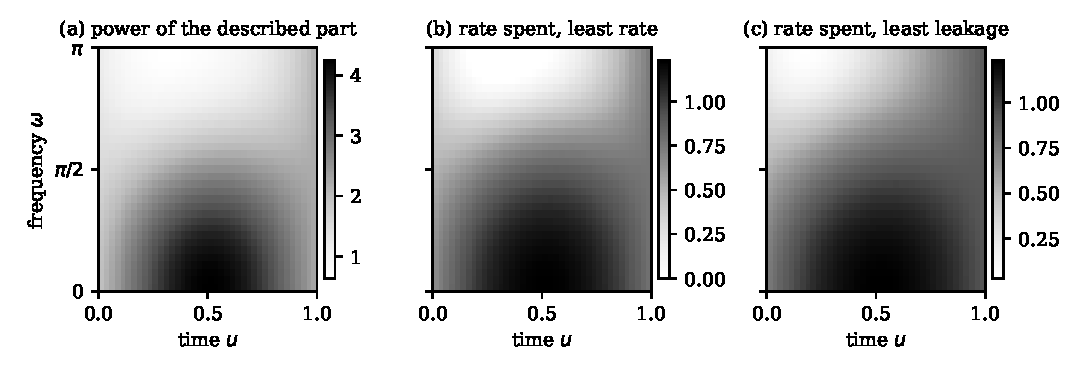
\includegraphics[width=\linewidth]{fig_ls.pdf}
\caption{A locally stationary source in $\R^2$ at $D=0.35D_{\max}$. (a) The
power $\tr\tilde Q(u,\omega)$ of the described combination over time
and frequency. (b) The rate that the description of least rate spends
at each time and frequency, in bits. It follows the power and leaves
the white region undescribed. (c) The same for the description of
least leakage, which describes the whole plane and spends more late in
time. Darker is larger in all three panels.}
\label{fig:ls}
\end{figure}

\noindent At $D=0.35D_{\max}$ the
description of least rate has rate $0.681$ and leakage $0.379$ bits per
symbol. It leaves $4\%$ of the time--frequency plane undescribed, the
high frequencies early in time, where the power of the described
combination is below the water level. The description of least leakage
has rate $0.775$ and leakage $0.313$. It describes the whole plane and
moves rate toward the end of the time axis: the second half of the
time axis receives $55\%$ of the rate of the first description and
$57\%$ of the rate of the second. One level governs each description
over the whole plane. The window costs of the source itself approach
these values: the least rate of the window is $0.6879$, $0.6842$, and
$0.6827$ at $N=16$, $32$, and $64$, against $0.6812$, and the least
leakage is $0.3143$, $0.3132$, and $0.3129$, against $0.3127$. The
stationary source with the time-averaged spectrum has least rate
$0.698$ and least leakage $0.323$, both larger, as the next corollary
shows in general. The numbers are computed by
\texttt{example\_ls.py} (Appendix~\ref{app:numver}).



\begin{corollary}\label{cor:lsavg}
Let the source be locally stationary and let
$\bar\Sigma(\omega)=\int_0^1\Sigma(u,\omega)\,du$, with spectral cost
$\bar V$ and region $\bar{\mathcal R}$. Then the two sources have the
same $D_{\max}$, and for every $\alpha\in[0,1]$ and $0<D<D_{\max}$
\[
\Vls(\alpha,D)\le\bar V(\alpha,D),\qquad\text{so that}\qquad\bar{\mathcal R}(D)\subseteq\mathcal R_{\mathrm{ls}}(D).
\]
\end{corollary}

\begin{proof}
Let $\bar\Sigma_B=\tfrac1B\sum_b\Sigma(b/B,\cdot)$. For each $n$ the
sources of period $n$ of the spectra $\Sigma(b/B,\cdot)$ and of
$\bar\Sigma_B$ have block-circulant covariances with a common Fourier
basis, and the covariance of the last is the average of the others.
By Corollary~\ref{cor:mixing}, the frontier cost per symbol of the
source of period $n$ of $\bar\Sigma_B$ at $D$ is at least
$\tfrac1B\sum_bV_{n,b}(\alpha,D^{(n)}_b)$ for some allocation with
$\tfrac1B\sum_bD^{(n)}_b\le D$, where $V_{n,b}$ is the cost per symbol of
the source of period $n$ of $\Sigma(b/B,\cdot)$. Let $n\to\infty$ along
a subsequence on which the allocations converge, to $(D^\ast_b)$. The
costs $V_{n,b}(\alpha,\cdot)$ are convex and nonincreasing and converge
pointwise to $V_{b/B}(\alpha,\cdot)$, by item~(iii) and, at and beyond the
maximal distortion, by the proof of \cite[Lemma~11(c)]{part2}. So the
convergence is uniform on compact subsets of $(0,\infty)$, and for
every $\epsilon>0$ the limit inferior of $V_{n,b}(\alpha,D^{(n)}_b)$ is
at least $V_{b/B}(\alpha,\max\{D^\ast_b,\epsilon\})$. By \eqref{eq:vB} the
spectral cost $\bar V_B$ of $\bar\Sigma_B$ satisfies
$\bar V_B(\alpha,D)\ge V_{\mu_B}(\alpha,D+\epsilon)$, hence
$\bar V_B(\alpha,D)\ge V_{\mu_B}(\alpha,D)$ by continuity. As
$B\to\infty$, $\bar\Sigma_B\to\bar\Sigma$ uniformly and
$\bar\Sigma\succeq aI$, so $\bar V_B\to\bar V$ by item~(iv) and the
continuity of $\bar V$ in the distortion, and $V_{\mu_B}\to\Vls$.
\end{proof}

\subsection{Sources that become stationary}

\begin{corollary}\label{cor:as}
Let $(T_t)_{t\ge1}$ be a centered Gaussian process in $\R^p$ whose
windows $T^N$ have covariances $\mathsf S_N$ that satisfy (L3), with the
time-invariant parties of this section. Let $\Sigma$ be a continuous
positive definite spectral density, with the symmetry of (L1), such
that for every $\eta>0$ there is $t_0$ with
\[
\bigl\|\mathsf S[I]-T_{|I|}(\Sigma)\bigr\|\le\eta
\]
for every set $I$ of consecutive times after $t_0$, where
$\mathsf S[I]$ is the covariance of $(T_t)_{t\in I}$. Let
$D_{\max}=\int\tr(Q\Sigma)\,\dw$. Then for
$0<D<D_{\max}$ the operational region is the spectral region
$\mathcal R(D)$ of $\Sigma$, and deterministic encoders suffice.
\end{corollary}

\begin{proof}
Fix $\eta$ with $0<\eta<a$, where $\Sigma\succeq aI$, small enough
that $D<(1-\eta/a)D_{\max}$, and $t_0$ as in the hypothesis. Use the two blocks $I_1=\{1,\dots,t_0\}$ and
$I_2=\{t_0+1,\dots,N\}$ in the proof of Theorem~\ref{thm:ls}, with
$\Sigma'=(1-\eta/a)\Sigma$ for the second block and nothing for the
first. For the converse, Lemma~\ref{lem:blocks} and the nonnegativity
of the cost of the first block give
$N[\alpha R_N+(1-\alpha)L_N]\ge(N-t_0)\mathsf V_{\mathsf S[I_2]}(\alpha,D_2)-c_1\chi$
with $(N-t_0)D_2\le ND_N$, and the comparison with $V$ is as there.
For the achievability, reproduce zero on the first block, at a cost in
distortion of at most $t_0\,b_0\tr Q/N$, and on the second block
repeat a code for the stationary source with spectral density
$\Sigma'$ on sub-blocks, through Lemma~\ref{lem:seeds}, as in that
proof. The set $\mathcal B(D)$ is the spectral
region of $\Sigma'$, and the argument ends as before.
\end{proof}

For example, let $T_t=X_t+E_t$ with $X$ a stationary Gaussian process
with a continuous positive definite spectral density and
$\sum_\tau\tau\|R(\tau)\|_{\fro}^2<\infty$, and $E$ an independent centered
Gaussian process with $\sum_t\E\|E_t\|^2<\infty$. The covariance of a
window after $t_0$ exceeds that of $X$ by a positive semidefinite
matrix of trace at most $\sum_{t>t_0}\E\|E_t\|^2$. For (L3), the
cross-covariance across a cut is the sum of those of $X$ and of $E$,
with squared Frobenius norms at most
$\sum_\tau\tau\|R(\tau)\|_{\fro}^2$ and $(\sum_t\E\|E_t\|^2)^2$. A
stable linear system with such a stationary output, started from a
state whose covariance exceeds the stationary one, is of this form,
with $E_t$ the response to the excess of the initial state. For the rate--distortion function of
asymptotically stationary Gaussian sources, defined through the
asymptotic equivalence of covariance matrices, see
\cite{gutierrez2018}.

\section{Cyclostationary Gaussian Processes}
\label{sec:cyclo}

A cyclostationary source varies with a period that does not grow with
the blocklength, so no stretch of time is long enough to look
stationary and Theorem~\ref{thm:ls} does not apply. Its statistics are
exactly periodic, and that is enough.

Fix a period $q\ge1$. Let $(T_t)_{t\in\mathbb Z}$ be a centered
Gaussian process in $\R^p$ whose covariances
$R_t(\tau)=\E[T_{t+\tau}T_t^{\mathsf T}]$ satisfy
$R_{t+q}(\tau)=R_t(\tau)$. The decoder's data may vary with the phase:
$Y_t=F_tT_t$ with $F_t$ of full row rank, weight $W_t\succ0$, and
$Q_t=F_t^{\mathsf T}W_tF_t$, all of period $q$ in $t$. The holder
observes
\[
S_t=\sum_kH_{t,k}T_{t-k}+U_t ,
\]
with real taps of period $q$ in $t$ and a centered Gaussian noise
process $U$ in $\R^r$, independent of $T$, whose covariances have period
$q$. The sum is a limit in mean square, as in \cite{part2}. A
code of blocklength $N$ acts on $T^N=(T_1,\dots,T_N)$, the holder is
given $S^N$, and rate, distortion, leakage, and $\mathcal A(D)$ are as
in \cite{part2}, with the weight $W_t$ at time $t$.

Stack one period at a time. For $j\in\mathbb Z$ let
\[
\tilde T_j=\bigl(T_{(j-1)q+1},\dots,T_{jq}\bigr)\in\R^{pq},
\]
and define $\tilde S_j$ and $\tilde U_j$ in the same way. The process
$(\tilde T_j)$ is stationary and Gaussian \cite{gladyshev1961}. Block
$(a,b)$ of its autocovariance at lag $j$ is $R_b(jq+a-b)$, for
$a,b\in\{1,\dots,q\}$. The holder's stacked observation is
$\tilde S_j=\sum_l\tilde H_l\tilde T_{j-l}+\tilde U_j$, where block
$(a,b)$ of $\tilde H_l$ is $H_{a,\,a-b+lq}$. The stacked weight is
$\tilde Q=\operatorname{diag}(Q_1,\dots,Q_q)$, which is
$\tilde F^{\mathsf T}\tilde W\tilde F$ for the block-diagonal matrices
of the $F_a$ and the $W_a$. We assume that the
stacked data satisfy the hypotheses of \cite{part2}: the spectral
densities $\tS(\omega)$ of $\tilde T$ and $\tS_U(\omega)$ of $\tilde U$
are continuous and positive definite, and the stacked filter has a
continuous frequency response. Let $\tilde V(\alpha,D)$ and
$\tilde{\mathcal R}(D)$ be the spectral cost and region of \cite{part2}
for the stacked data, per stacked symbol, and let
\begin{equation}
V_{\mathrm{cs}}(\alpha,D)=\tfrac1q\tilde V(\alpha,qD),\qquad
D_{\max}=\tfrac1q\sum_{a=1}^q\tr\bigl(Q_aR_a(0)\bigr),\qquad
\bar d=\max_a\tr\bigl(Q_aR_a(0)\bigr),
\label{eq:vcs}
\end{equation}
with $\mathcal R_{\mathrm{cs}}(D)$ the set of pairs with
$\alpha R+(1-\alpha)L\ge V_{\mathrm{cs}}(\alpha,D)$ for every $\alpha$.

\begin{theorem}\label{thm:cyclo}
Let $0<D<D_{\max}$.
\begin{enumerate}
\item[(a)] $\mathcal A(D)=\mathcal R_{\mathrm{cs}}(D)$, and deterministic
encoders suffice.
\item[(b)] The region is unchanged when the holder has its observations
on any sets of times that contain the windows, in particular its
whole observation process.
\item[(c)] The region is unchanged when the windows start at any other
phase of the period.
\item[(d)] If the holder's map is memoryless, $S_t=H_tT_t+U_t$ with
$U_t$ independent across time, then every code of blocklength $N$
satisfies
$\alpha R_N+(1-\alpha)L_N\ge V_{\mathrm{cs}}(\alpha,D_N+q\bar d/N)$ for
every $\alpha$, and $\alpha R_N+(1-\alpha)L_N\ge V_{\mathrm{cs}}(\alpha,D_N)$
when $q$ divides $N$. The window cost at $N=kq$, which is the window
cost of size $k$ of the stacked process at distortion $qD$ divided by
$q$, is at least $V_{\mathrm{cs}}(\alpha,D)$ and converges to it, with a
gap of order $1/N$ when $\tS$ is Lipschitz.
\end{enumerate}
\end{theorem}

\begin{proof}
A code of blocklength $kq$ for the process is a code of blocklength
$k$ for the stacked process with the same message. Its rate and
leakage per symbol are those of the stacked code divided by $q$, and
so is its distortion, because the stacked distortion with the weight
$\tilde Q$ is the sum of the distortions of the $q$ symbols of a
period. So the closure of the set of pairs achievable at $D$ with
blocklengths that are multiples of $q$ is
$\tfrac1q\tilde{\mathcal A}(qD)$, which is
$\tfrac1q\tilde{\mathcal R}(qD)=\mathcal R_{\mathrm{cs}}(D)$ by item~(i) of
Section~\ref{sec:model}, with deterministic encoders.

Let a code have blocklength $N=kq+s$ with $0<s<q$. Extend it to
blocklength $N'=(k+1)q$: the encoder ignores the last $q-s$ symbols
and the decoder reproduces zero for them. The message is unchanged, so
the rate per symbol is $R_NN/N'\le R_N$. The holder now has $S^{N'}$,
which contains $S^N$, so the leakage per symbol is at most
$L_NN/N'\le L_N$. The distortion is at most
$(ND_N+(q-s)\bar d)/N'\le D_N+q\bar d/N$. Hence a pair achievable at
$D$ is achievable at $D$ with blocklengths that are multiples of $q$.
This proves (a).

(b) A holder with more observations has a leakage no larger, so every
pair achievable against the holder of (a) is achievable against it.
For the other direction let a code of blocklength $N$ be given, with
the holder's observations on a finite set of times $\mathcal T$ that
contains the window. Extend the code to the blocklength $N'$, the next
multiple of $q$, as in (a), and let $\mathcal T''$ be a union of whole
periods that contains $\mathcal T$ and $\{1,\dots,N'\}$. By
\cite[Theorem~23]{part2} for the stacked process, whose window of size
$N'/q$ is $\{1,\dots,N'\}$,
\[
H\bigl(M\mid S^{N'}\bigr)\le H\bigl(M\mid S_{\mathcal T''}\bigr)+o(N)\le H\bigl(M\mid S_{\mathcal T}\bigr)+o(N),
\]
with a term $o(N)$ that does not depend on the code. So the extended
code, against the holder of (a), has a leakage per symbol at most that
of the given code plus $o(1)$, a rate no larger, and a distortion
larger by at most $q\bar d/N$. An infinite set of times is handled by
the infimum over its finite subsets, as in \cite{part2}.

(c) Let $\mathcal A^{(c)}(D)$ be the region for windows that start at
time $1+c$. A code for the window $\{1+c,\dots,N+c\}$ becomes a code
for $\{1,\dots,N+c\}$ when the first $c$ symbols are ignored and
reproduced by zero. As above its rate and leakage do not increase and
its distortion increases by at most $c\bar d/N$. So
$\mathcal A^{(c)}(D)\subseteq\mathcal A^{(0)}(D)$ for $0\le c\le q$, and in
the same way $\mathcal A^{(q)}(D)\subseteq\mathcal A^{(c)}(D)$. The
process shifted by $q$ has the law of the process, so
$\mathcal A^{(q)}(D)=\mathcal A^{(0)}(D)$.

(d) The stacked holder map is memoryless with white noise, so item~(ii)
of Section~\ref{sec:model} applies to the stacked process and gives the
statements for $N=kq$, the rate of convergence being that of
\cite[Theorem~15(b),(c)]{part2}. For other $N$ apply the bound to the
extended code, whose weighted cost is no larger, and use that
$V_{\mathrm{cs}}$ is nonincreasing in the distortion.
\end{proof}

\subsection{The harmonic form}

Suppose $\sum_\tau\|R_t(\tau)\|<\infty$ for every $t$. The cyclic
autocovariances and cyclic spectra of the process are
\[
B_k(\tau)=\frac1q\sum_{t=1}^qR_t(\tau)e^{-2\pi ikt/q},\qquad
f_k(\lambda)=\sum_\tau B_k(\tau)e^{-i\lambda\tau},
\]
for $k$ modulo $q$, so that
$R_t(\tau)=\sum_{k=0}^{q-1}B_k(\tau)e^{2\pi ikt/q}$. The function $f_0$ is
the spectral density of the stationary process with the time-averaged
autocovariance $B_0$. For $\omega\in[-\pi,\pi]$ let
$\lambda_k(\omega)=(\omega+2\pi k)/q$, $k=0,\dots,q-1$. These are $q$
frequencies of the original time axis that differ by multiples of the
cycle frequency $2\pi/q$. Let $\mathsf V(\omega)$ be the $pq\times pq$
matrix with blocks $q^{-1/2}e^{ia\lambda_k(\omega)}I_p$ in block row
$a\in\{1,\dots,q\}$ and block column $k$.

\begin{proposition}\label{prop:harmonic}
$\mathsf V(\omega)$ is unitary, and
\[
\mathsf V(\omega)^{\herm}\,\tS(\omega)\,\mathsf V(\omega)=\cF(\omega),
\]
the matrix whose block $(k,l)$ is $f_{k-l}\bigl(\lambda_k(\omega)\bigr)$,
with the index $k-l$ taken modulo $q$. If the decoder's weight and the
holder are time-invariant, $Q_t=Q$ and $S_t=HT_t+U_t$ with white noise
of covariance $\Sigma_U$, then
\begin{equation}
V_{\mathrm{cs}}(\alpha,D)=\min\Bigl\{\int_{-\pi/q}^{\pi/q}\phi_{\alpha,\lambda}\bigl(X(\lambda)\bigr)\dl:\
\int_{-\pi/q}^{\pi/q}\tr\Bigl(\cF^{1/2}(I_q\otimes Q)\cF^{1/2}X(\lambda)\Bigr)\dl\le D\Bigr\}
\label{eq:coset}
\end{equation}
over Hermitian fields $0\prec X(\lambda)\preceq I_{pq}$, where $\cF$ is
evaluated at $\omega=q\lambda$ and $\phi_{\alpha,\lambda}$ is the weighted
per-frequency cost of \cite{part2} for the source matrix $\cF$, the
weight $I_q\otimes Q$, and the holder
$(I_q\otimes H,I_q\otimes\Sigma_U)$. The same holds for a time-invariant
filter and stationary noise, with $H$ and $\Sigma_U$ replaced by
$\operatorname{diag}_k\bigl(H(\lambda_k)\bigr)$ and
$\operatorname{diag}_k\bigl(\Sigma_U(\lambda_k)\bigr)$.
\end{proposition}

\begin{proof}
Block $(k,l)$ of $\mathsf V^{\herm}\mathsf V$ is
$\tfrac1q\sum_ae^{-2\pi ia(k-l)/q}I_p$, which is $I_p$ for $k=l$ and zero
otherwise. Block $(a,b)$ of $\tS(\omega)$ is
$\sum_jR_b(jq+a-b)e^{-i\omega j}$. Put $\tau=jq+a-b$. For fixed $b$ the
pairs $(j,a)$ correspond one to one to the integers $\tau$, and
$a\lambda_k+\omega j=\lambda_k(\tau+b)-2\pi kj$. So block $(k,l)$ of
$\mathsf V^{\herm}\tS\mathsf V$ is
\[
\frac1q\sum_{b=1}^q\sum_\tau\sum_mB_m(\tau)e^{2\pi imb/q}e^{-i\lambda_k(\tau+b)}e^{ib\lambda_l}
=\sum_m\Bigl[\sum_\tau B_m(\tau)e^{-i\lambda_k\tau}\Bigr]\frac1q\sum_{b=1}^qe^{2\pi ib(m-k+l)/q},
\]
and the last sum is $q$ when $m\equiv k-l$ modulo $q$ and zero
otherwise. For time-invariant parties
$\mathsf V=\mathsf v\otimes I_p$ with a $q\times q$ unitary $\mathsf v$,
so $\mathsf V^{\herm}(I_q\otimes Q)\mathsf V=I_q\otimes Q$ and
$(I_q\otimes H)\mathsf V=(\mathsf v\otimes I_r)(I_q\otimes H)$, and the
per-frequency costs of \cite{part2}, which are unchanged by a unitary
change of coordinates of the source and of the observation, are those
stated. The change of variable $\omega=q\lambda$ turns
$\tfrac1q\int_{-\pi}^{\pi}\cdot\,\dw$ into
$\int_{-\pi/q}^{\pi/q}\cdot\,\dl$. For a filter, the same computation with
the taps $H_{a-b+lq}$ in place of $R_b(jq+a-b)$ shows that the stacked
response is
$(\mathsf v\otimes I_r)\operatorname{diag}_k(H(\lambda_k))(\mathsf v\otimes I_p)^{\herm}$,
and likewise for the noise spectrum.
\end{proof}

The problem at a coset is a matrix problem of size $pq$. The diagonal
blocks of $\cF$ are the time-averaged spectrum at the $q$ frequencies
of the coset, and the off-diagonal blocks are the cyclic spectra,
which correlate components of the process at frequencies that differ
by multiples of $2\pi/q$. In \cite{part2} the frequencies are coupled
only through the water level. Here they are coupled within a coset
through the source, and across cosets through the level.

\begin{corollary}\label{cor:blocking}
If the process is stationary and the parties are time-invariant, so
that the data are those of \cite{part2}, then for every $q$ the cost
$V_{\mathrm{cs}}$ and the region $\mathcal R_{\mathrm{cs}}$ computed
with period $q$ equal $V$ and $\mathcal R$ of \cite{part2}.
\end{corollary}

\begin{proof}
The stacked data meet the assumptions of this section. Consider the matrix function with blocks
\[
\tfrac1q\sum_k\Sigma\bigl(\lambda_k(\omega)\bigr)e^{i(a-b)\lambda_k(\omega)} .
\]
It is continuous, and its Fourier coefficients are $R(jq+a-b)$ by the
change of variable $\lambda=(\omega+2\pi k)/q$, so it is $\tS(\omega)$.
Hence
\[
\tS=\mathsf V\operatorname{diag}_k\bigl(\Sigma(\lambda_k)\bigr)\mathsf V^{\herm},
\]
which is positive definite. The same holds for the filter and the noise
spectrum. No summability is needed. Both regions are then the
operational region of the same source with the same codes, by
Theorem~\ref{thm:cyclo}(a) and item~(i) of Section~\ref{sec:model}, and a
closed convex upward closed region determines its support values.
\end{proof}

In this case the matrix $\cF$ is block-diagonal with blocks
$\Sigma(\lambda_k)$, by the identity in the proof, and the corollary
also follows from \eqref{eq:coset} and the splitting of the problem
along subspaces invariant under the weight and the holder's
information \cite[Theorem~12]{part1}.

\begin{remark}
A stationary process seen through periodically varying parties is
covered by the same theorem. If $T_t=c_tX_t$ for a scalar stationary
Gaussian process $X$ with a continuous positive spectral density and
real $c_t\ne0$ of period $q$, the stacked spectrum is
$\mathsf C\,\tS_X\,\mathsf C$ with $\mathsf C=\operatorname{diag}(c_a)$,
which is continuous and positive definite, and the problem for $T$
with a time-invariant weight $Q$ and a memoryless holder map $H$ is the
problem for $X$ with the weight $c_t^2Q$ and the holder map $c_tH$.
\end{remark}

\subsection{The phase-averaged spectrum}

Averaging the covariances of a cyclostationary process over the phase
of the cycle gives the autocovariance $B_0$ of a stationary process,
with spectral density $f_0$. The stationary Gaussian source with that
spectral density is a different source. It is not the cyclostationary
source seen by a party that does not know the phase: a cyclostationary
Gaussian process with a random phase is a mixture, which is not
Gaussian. The next theorem compares the optimal costs of the two
Gaussian sources. It does not give the operational penalty of not
knowing the phase. Let
$V_0$ and $\mathcal R_0$ be the spectral cost and region of
\cite{part2} for the spectral density $f_0$.

\begin{theorem}\label{thm:averaged}
Let the process have a continuous positive definite stacked spectral
density, as assumed in this section, and summable covariances, as in
Proposition~\ref{prop:harmonic}. Let the decoder's weight and the
holder be time-invariant: $Q_t=Q$, and the holder has a filter with a
continuous frequency response $H(\lambda)$ and stationary noise with a
continuous positive definite spectral density, so that the stacked
filter and noise meet the assumptions of this section by the last
statement of Proposition~\ref{prop:harmonic}. Then $f_0$ is
continuous and positive definite, the two sources have the same
$D_{\max}$, and for every $\alpha\in[0,1]$ and $0<D<D_{\max}$
\[
V_{\mathrm{cs}}(\alpha,D)\le V_0(\alpha,D),\qquad\text{so that}\qquad
\mathcal R_0(D)\subseteq\mathcal R_{\mathrm{cs}}(D).
\]
\end{theorem}

\begin{proof}
The blocks $f_0(\lambda_k(\omega))$ are the diagonal blocks of the
positive definite matrix $\cF(\omega)$, and every frequency is some
$\lambda_k(\omega)$, so $f_0\succ0$. It is continuous because $B_0$ is
summable, and $\int\tr(Qf_0)\,\dl=\tr(QB_0(0))=D_{\max}$.

Let $n=n'q$, and let $\mathsf S_n$ be the covariance of the source of
period $n'$ of the stacked process, a real matrix of size $pn$. By
item~(iii) of Section~\ref{sec:model}, applied to the stacked data, its
cost per symbol of the original time axis tends to
$V_{\mathrm{cs}}(\alpha,D)$ as $n'\to\infty$. Let $\mathsf U_n$ be the
unitary matrix of the Fourier transform on $n$ points, with the points
indexed by the times $1,\dots,n$. The product of the Fourier transform
on $n'$ points of the stacked axis with $\mathsf V(\omega_j)$,
$\omega_j=2\pi j/n'$, is $\mathsf U_n$ with its columns arranged by
cosets, because
$e^{i\omega_jj'}e^{ia\lambda_k(\omega_j)}=e^{i\lambda_k(\omega_j)(j'q+a)}$
and the frequencies $\lambda_k(\omega_j)=2\pi(j+n'k)/n$ are the $n$
Fourier frequencies. So $\mathsf U_n^{\herm}\mathsf S_n\mathsf U_n$ has
the blocks of $\cF(\omega_j)$ between frequencies of one coset and
zero blocks between cosets. By Proposition~\ref{prop:harmonic} the
holder's matrix and the noise covariance of this source are the
block-circulant matrices on $n$ points with the symbols $H$ and
$\Sigma_U$, so its information matrix $J_n$ is block-circulant on $n$
points, and so is the weight $\tfrac1nI_n\otimes Q$.

Let $\mathsf P$ be the cyclic shift by one symbol on $n$ points, a real
orthogonal matrix that commutes with every block-circulant matrix on
$n$ points. In the Fourier basis, conjugation by $\mathsf P^c$
multiplies the block between the frequencies $2\pi\kappa/n$ and
$2\pi\kappa'/n$ by a factor $e^{\pm2\pi ic(\kappa-\kappa')/n}$, with a
sign fixed by the convention. Within a coset
$\kappa-\kappa'=n'(k-l)$, so the factor is $e^{\pm2\pi ic(k-l)/q}$, and
the average over $c=0,\dots,q-1$ removes the blocks with $k\ne l$. Hence
\[
\bar{\mathsf S}_n=\frac1q\sum_{c=0}^{q-1}\mathsf P^c\,\mathsf S_n\,\mathsf P^{-c}
\]
is the block-circulant matrix on $n$ points with eigen-blocks
$f_0(2\pi\kappa/n)$, the covariance of the source of period $n$ of the
stationary process with spectral density $f_0$. By
Corollary~\ref{cor:mixing} with $O_c=\mathsf P^c$,
$\VG(\alpha,D;\bar{\mathsf S}_n)\ge\VG(\alpha,D;\mathsf S_n)$ for the
common weight and information matrix. These are costs of the whole
block. Divided by $n$, the left side tends to $V_0(\alpha,D)$ as
$n'\to\infty$, by item~(iii) for $f_0$, and the right side to
$V_{\mathrm{cs}}(\alpha,D)$.
\end{proof}

So the cyclostationary source costs no more, at any weight, than the
stationary source with the phase-averaged spectrum. The inequality
compares two Gaussian sources and their best descriptions. It does not
say how a code designed for the averaged source performs on the
cyclostationary one. Its proof uses the mixture
of the $q$ phase shifts of the cyclostationary source, which is not
Gaussian. In the instance recorded in Appendix~\ref{app:numver}, with
$q=2$ and a scalar source, the saving is $0.023$ bits per symbol at
$D=0.1D_{\max}$ and at $D=0.4D_{\max}$, for the rate and for the leakage.

\section{Independent Stationary Regimes}
\label{sec:regimes}

Theorem~\ref{thm:ls} asks for a spectrum that is continuous in time.
A source that jumps between regimes is not covered, and for
independent regimes the answer is immediate from \cite{part1}.

Let $(\Sigma_i,Q_i,H_i,\Sigma_{U,i})$, $i=1,\dots,k$, be the data of $k$
stationary Gaussian sources as in \cite{part2}, all in $\R^p$, each
with a memoryless holder map and white noise, and let
$\rho_1,\dots,\rho_k>0$ be rational with sum one. For blocklengths
$N$ such that every $\rho_iN$ is an integer, the source emits a
window made of $k$ consecutive segments of lengths $\rho_iN$, the
$i$th being a window of the $i$th process with its holder's
observations, and the segments are independent. Let $V_i$ be the
spectral cost of the $i$th source and
\[
V_{\mathrm{mix}}(\alpha,D)=\min\Bigl\{\sum_i\rho_iV_i(\alpha,D_i):\ \sum_i\rho_iD_i\le D\Bigr\},
\]
with $\mathcal R_{\mathrm{mix}}(D)$ the corresponding region and
$D_{\max}=\sum_i\rho_iD_{\max,i}$.

\begin{proposition}\label{prop:regimes}
For $0<D<D_{\max}$ the operational region of the source with
independent regimes is $\mathcal R_{\mathrm{mix}}(D)$. The minimum in
$V_{\mathrm{mix}}$ is attained by the fields that solve the fixed
point equation of \cite[Theorem~4]{part2} in every regime and at every
frequency with one common level. The achievability holds whatever the
dependence between the segments.
\end{proposition}

\begin{proof}
\emph{Converse.} Apply the proof of Lemma~\ref{lem:blocks} with the
segments as blocks. The two cut terms $\mathsf c(T)$ and
$\mathsf c(T\mid S)$ vanish because the pairs formed by a segment and
its observations are independent, and the step for a block uses only
the weight and the holder of that block, which may differ between the
segments. With item~(ii) of Section~\ref{sec:model}, a code of
blocklength $N$ with distortion $D_i$ per symbol in segment $i$ has
weighted cost at least $\sum_i\rho_iV_i(\alpha,D_i)$, which is at least
$V_{\mathrm{mix}}(\alpha,D_N)$. Each $V_i(\alpha,\cdot)$ is convex, nonincreasing, and
unbounded as the distortion tends to zero, so
$V_{\mathrm{mix}}(\alpha,\cdot)$ is convex and nonincreasing, hence
continuous, and the bound passes to achievable pairs.

\emph{Achievability.} Take codes for the $i$th source of blocklength
$\rho_iN$, which exist at every large blocklength by item~(i) for
every pair of its region, and the code with one message beyond its
maximal distortion. Use them on the segments, with the tuple of
messages. The rate and the distortion are the averages with weights
$\rho_i$, and
$H(M\mid S^N)\le\sum_iH(M_i\mid S^N)\le\sum_iH(M_i\mid S_i)$, where $S_i$
is the holder's observation of the $i$th segment. Neither step uses
independence between the segments. So every pair of the set
\[
\mathcal B(D)=\text{closure of }\bigcup\Bigl\{\sum_i\rho_i\mathcal R_i(D_i):\ \sum_i\rho_iD_i\le D\Bigr\}
\]
is achievable, where $\mathcal R_i$ is the region of the $i$th source
and the sum is the Minkowski sum. As in the proof of
Theorem~\ref{thm:ls}, $\mathcal B(D)$ is closed, convex, and upward
closed, and its support value at $(\alpha,1-\alpha)$ is at most
$V_{\mathrm{mix}}(\alpha,D)$, so it contains
$\mathcal R_{\mathrm{mix}}(D)$.

\emph{One level.} The program for $V_{\mathrm{mix}}$ is the program of
item~(v) on the disjoint union of $k$ circles with the measure that
gives the $i$th circle mass $\rho_i$, after the holders' observations
are padded to a common dimension by coordinates of pure noise, which
does not change their information matrices.
\end{proof}

When the segments are dependent the converse can fail. If the second
segment repeats the first, half the rate suffices. Under the cut
condition (L3) the converse holds again, by Lemma~\ref{lem:blocks}, so
a Gaussian source that switches between stationary regimes at a
bounded number of times, with common parties and bounded correlation
across every cut, has the region $\mathcal R_{\mathrm{mix}}(D)$ when its
segments have the covariances of the regimes.

\section{Unstable Autoregressive Sources}
\label{sec:unstable}

Condition (L3) bounds the covariance, and so excludes every source whose
variance grows without bound. The simplest such sources are
autoregressive sources with unstable poles. For a scalar source of this
kind with the memoryless holder in white noise, the region is the
spectral region of a stationary source moved by a constant: each
unstable pole costs the logarithm of its modulus in rate, and it costs
nothing in leakage when the holder observes the source.

Let $d\ge1$, let $\phi_1,\dots,\phi_d$ be real, and let
\[
T_t=\sum_{i=1}^d\phi_iT_{t-i}+\xi_t\quad(t\ge1),\qquad T_t=0\quad(t\le0),
\]
with $\xi_t$ independent $\mathcal N(0,\sigma^2)$, $\sigma^2>0$. Write
$\phi(z)=1-\sum_i\phi_iz^i=\prod_{i=1}^d(1-\rho_iz)$, so that
$\rho_1,\dots,\rho_d$ are the poles, and assume that no pole lies on the
unit circle. The source is scalar, $Y_t=FT_t$ with $F\ne0$, the weight
is $W>0$, and $Q=F^2W$. The holder observes $S_t=HT_t+U_t$ with $H\in\R$
and $U_t$ independent $\mathcal N(0,\sigma_U^2)$, $\sigma_U^2>0$, and
$J=H^2/\sigma_U^2$. A code of blocklength $N$ acts on $T^N$ as in
Section~\ref{sec:model}, with private randomness allowed, and
achievable pairs and $\mathcal A(D)$ are defined as in
Section~\ref{sec:ls}. Let
\[
\rho_\star=\sum_{i:\,|\rho_i|>1}\log|\rho_i|,\qquad
f(\omega)=\frac{\sigma^2}{|\phi(e^{i\omega})|^2},
\]
and let $V_f$ and $\mathcal R_f(D)$ be the spectral cost and region of
Section~\ref{sec:model} for the stationary scalar source with spectral
density $f$, the weight $Q$, and the holder $(H,\sigma_U^2)$, with
$\mathcal R_f(D)$ the nonnegative quadrant for
$D\ge D_{\max}^f=Q\int f\,\dw$. Since
$|1-\rho e^{i\omega}|=|\rho|\,|1-\overline{\rho}^{\,-1}e^{i\omega}|$, the
function $f$ is the spectral density of the stable autoregressive process
whose poles are $\rho_i$ when $|\rho_i|<1$ and $1/\overline{\rho_i}$ when
$|\rho_i|>1$, driven by noise of variance $\sigma^24^{-\rho_\star}$.

\begin{lemma}\label{lem:separable}
Let $T$ be a centered Gaussian vector of $n$ scalar symbols with
covariance $\mathsf S\succ0$ and eigenvalues
$\lambda_1\ge\dots\ge\lambda_n$, with the weight $Q$ and the holder
$(H,\sigma_U^2)$ above. For $0<D<\tfrac Qn\tr\mathsf S$,
\[
\mathsf V_{\mathsf S}(\alpha,D)=\frac1n\min\Bigl\{\sum_{k=1}^nc_\alpha(\lambda_k,\delta_k):\ 0<\delta_k\le\lambda_k,\ \frac Qn\sum_{k=1}^n\delta_k\le D\Bigr\},
\qquad
c_\alpha(\lambda,\delta)=\frac12\log\frac\lambda\delta+\frac{1-\alpha}2\log\frac{1+J\delta}{1+J\lambda}.
\]
Here $c_\alpha=\alpha r+(1-\alpha)\ell$ with $r=\tfrac12\log(\lambda/\delta)$
and $\ell=\tfrac12\log\frac{1/\delta+J}{1/\lambda+J}$, and $0\le\ell\le r$,
with $\ell=r$ when $H=0$. Both $r$ and $\ell$ are convex in the ratio
$\delta/\lambda$. For every $\alpha$ the minimum is attained at the same
allocation
\[
\delta_k=\min\{\lambda_k,\theta\},\qquad\text{where }\theta>0\text{ solves }\ \frac Qn\sum_k\min\{\lambda_k,\theta\}=D,
\]
so the region of the vector problem is the quadrant above the rate and
the leakage per symbol of this allocation.
\end{lemma}

\begin{proof}
In \eqref{eq:costs}, with $K=\mathsf S$ and the information matrix
$JI_n$, $\det g(\Delta)=\det\Delta/\det(I+J\Delta)$, so
\[
\alpha r(\Delta)+(1-\alpha)\ell(\Delta)=\tfrac12\bigl(\log\det\mathsf S-\log\det\Delta\bigr)+\tfrac{1-\alpha}2\bigl(\log\det(I+J\Delta)-\log\det(I+J\mathsf S)\bigr).
\]
This and the constraint $\tfrac Qn\tr\Delta\le D$ depend on $\Delta$ only
through its eigenvalues $\delta_1\ge\dots\ge\delta_n$. If
$\Delta\preceq\mathsf S$ then $\delta_k\le\lambda_k$ for every $k$, by the
Courant--Fischer theorem, and conversely every such sequence is the
spectrum of $\Psi\,\mathrm{diag}(\delta)\Psi^{\mathsf T}\preceq\mathsf S$,
where $\Psi$ is orthogonal and $\Psi^{\mathsf T}\mathsf S\Psi$ is
diagonal. The bounds on $\ell$ follow from $\delta\le\lambda$ and
$\ell=r+\tfrac12\log\frac{1+J\delta}{1+J\lambda}$. With $x=\delta/\lambda$,
$r=-\tfrac12\log x$ and $\ell=\tfrac12\log(1/(\lambda x)+J)$ up to a
constant, and $x\mapsto\ln(a/x+J)$ has second derivative
$1/x^2-J^2/(a+Jx)^2\ge0$ for $a>0$.

For the common minimizer: up to terms that do not depend on $\delta$, the
objective is $\sum_k\varphi_\alpha(\delta_k)$ with
$\varphi_\alpha(\delta)=-\tfrac12\log\delta+\tfrac{1-\alpha}2\log(1+J\delta)$,
the same function for every $k$. It is strictly decreasing and strictly
convex: $2\ln2\,\varphi_\alpha'(\delta)=-1/\delta+(1-\alpha)J/(1+J\delta)<0$
and $2\ln2\,\varphi_\alpha''(\delta)=1/\delta^2-(1-\alpha)J^2/(1+J\delta)^2>0$.
A minimizer exists, because $\varphi_\alpha\to\infty$ as $\delta\to0$. It
uses the whole budget, since otherwise some $\delta_k<\lambda_k$ could be
raised. If $\delta_i<\min\{\lambda_i,\theta\}$ for some $i$, then, the
budgets being equal, $\delta_j>\min\{\lambda_j,\theta\}$ for some $j$, so
$\delta_j>\theta$ because $\delta_j\le\lambda_j$. Moving a small amount
from $\delta_j$ to $\delta_i$ keeps the allocation feasible and lowers the
objective, because $\varphi_\alpha'(\delta_i)<\varphi_\alpha'(\delta_j)$.
So $\delta_k\ge\min\{\lambda_k,\theta\}$ for every $k$, with equal sums,
and equality holds throughout. The allocation does not depend on
$\alpha$, so $\mathsf V_{\mathsf S}(\alpha,D)=\alpha\bar r+(1-\alpha)\bar\ell$
for the rate $\bar r$ and the leakage $\bar\ell$ per symbol of this
allocation, and the region, the set of pairs above every such line, is
the quadrant above $(\bar r,\bar\ell)$.
\end{proof}

\begin{lemma}\label{lem:arspec}
Let $\lambda_1\ge\dots\ge\lambda_N$ be the eigenvalues of the covariance
$\Gamma_N$ of $T^N$, and let $m_\phi$ and $M_\phi$ be the minimum and the
maximum of $|\phi(e^{i\omega})|^2$, so that $0<m_\phi\le M_\phi$.
\begin{enumerate}
\item[(a)] $\lambda_k\ge\sigma^2/M_\phi$ for every $k$, and
$\lambda_k\le\sigma^2/m_\phi$ for $k>d$.
\item[(b)] The probability measures $\mu_N$ that put mass $1/(N-d)$ on
each $\lambda_k$ with $k>d$ converge weakly to the law $\mu$ of
$f(\omega)$ for $\omega$ uniform on $[-\pi,\pi)$.
\item[(c)] $\frac1{2N}\sum_{k\le d}\log\lambda_k\to\rho_\star$.
\end{enumerate}
\end{lemma}

\begin{proof}
Let $A_N$ be the lower triangular $N\times N$ matrix with ones on the
diagonal and $-\phi_i$ on the $i$th subdiagonal. Then $A_NT^N=\xi^N$, so
$\Gamma_N=\sigma^2(A_N^{\mathsf T}A_N)^{-1}$ and $\lambda_k=\sigma^2/s_k$,
where $s_1\le\dots\le s_N$ are the eigenvalues of
$A_N^{\mathsf T}A_N$. Let $C$ be the $(N+d)\times N$ matrix of the full
convolution with $(1,-\phi_1,\dots,-\phi_d)$. Its first $N$ rows are
$A_N$; call its last $d$ rows $R$. Every column of $C$ contains all the
coefficients, so $C^{\mathsf T}C$ is the Toeplitz matrix
$T_N(|\phi|^2)$ of the symbol $|\phi(e^{i\omega})|^2$, and
\[
A_N^{\mathsf T}A_N=T_N(|\phi|^2)-R^{\mathsf T}R .
\]
Let $\tilde s_1\le\dots\le\tilde s_N$ be the eigenvalues of
$T_N(|\phi|^2)$. They lie in $[m_\phi,M_\phi]$, because
\[
x^{\mathsf T}T_N(|\phi|^2)x=\int\Bigl|\sum_tx_te^{it\omega}\Bigr|^2|\phi(e^{i\omega})|^2\,\dw .
\]
Since $R^{\mathsf T}R\succeq0$, $s_k\le\tilde s_k$ for every $k$. Since
its rank is at most $d$, $s_k\ge\tilde s_{k-d}$ for $k>d$: in the
max-min characterization of $s_k$, take the intersection of the kernel
of $R$ with a subspace of dimension $N-k+d+1$ that attains
$\tilde s_{k-d}$. This proves (a).

For (b) let $\psi$ be a bounded Lipschitz function on
$\mathcal I_\phi=[\sigma^2/M_\phi,\sigma^2/m_\phi]$. Then $x\mapsto\psi(\sigma^2/x)$ is
Lipschitz on $[m_\phi,M_\phi]$, so it has bounded variation, say $v$,
and sup norm, say $w$. Each point outside the finite set
$\{\tilde s_k\}$ lies in at most $d$ of the intervals
$[\tilde s_{k-d},\tilde s_k]$, and the variation of a Lipschitz function
puts no mass on a finite set, so
\[
\Bigl|\sum_{k>d}\psi(\lambda_k)-\sum_{k=1}^N\psi(\sigma^2/\tilde s_k)\Bigr|\le d\,(v+w).
\]
By Szeg\H{o}'s theorem \cite{grenander1958},
$\tfrac1N\sum_k\psi(\sigma^2/\tilde s_k)\to\int\psi(f)\,\dw$. Hence
$\int\psi\,d\mu_N\to\int\psi\,d\mu$ for every bounded Lipschitz $\psi$,
which is weak convergence.

For (c), $\det A_N=1$, so $\sum_k\log s_k=0$. The bound above with
$\log$ in place of $\psi(\sigma^2/\cdot)$, and Szeg\H{o}'s theorem, give
$\tfrac1N\sum_{k>d}\log s_k\to\int\log|\phi(e^{i\omega})|^2\dw$, which is
$2\rho_\star$ by Jensen's formula
$\int\log|1-\rho e^{i\omega}|\dw=\log\max\{1,|\rho|\}$. So
$\tfrac1N\sum_{k\le d}\log s_k\to-2\rho_\star$, and $\lambda_k=\sigma^2/s_k$
gives (c).
\end{proof}

\begin{theorem}\label{thm:unstable}
For every $D>0$,
\[
\mathcal A(D)=\bigl(\rho_\star,\ \rho_\star\mathbf 1_{\{H=0\}}\bigr)+\mathcal R_f(D),
\]
deterministic encoders suffice, and the converse holds also for
encoders with private randomness.
\end{theorem}

When the holder observes the source, the region of the unstable source
is the region of the stationary source with spectral density $f$ moved
by $\rho_\star$ in rate: every unstable pole is paid for in rate, and
none in leakage. When $H=0$ the leakage equals the rate and both move.
At every distortion the rate is at least $\rho_\star$, because the
variance of the source grows without bound.

With no holder, or at the weight that counts only the rate, the theorem
gives the rate--distortion function $\rho_\star+r_f(D)$ of an unstable
Gaussian autoregressive source. This is the form found by Hashimoto
and Arimoto \cite{hashimoto1980}. Gray \cite{gray1970} gave the
function in another form, and Gray and Hashimoto
\cite{grayhashimoto2008} showed that the two agree. For first-order
sources Tian and Kostina \cite{tian2019} prove coding theorems with
second-order terms. What is new here is the second cost.

\begin{proof}
\emph{Converse.} Let a code of blocklength $N$, with or without private
randomness, have distortion $D_N$. Section~\ref{sec:model} and
Lemma~\ref{lem:separable} give
$\alpha R_N+(1-\alpha)L_N\ge\tfrac1N\sum_kc_\alpha(\lambda_k,\delta_k)$
for some $\delta$ with $0<\delta_k\le\lambda_k$ and
$\tfrac QN\sum_k\delta_k\le D_N$; when $D_N\ge\tfrac QN\tr\Gamma_N$ take
$\delta=\lambda$, for which the sum is zero. Let
$\bar\alpha=\alpha+(1-\alpha)\mathbf 1_{\{H=0\}}$. For $k\le d$,
$c_\alpha(\lambda_k,\delta_k)\ge\bar\alpha\,r$ by Lemma~\ref{lem:separable},
and $\delta_k\le ND_N/Q$, so
\[
\frac1N\sum_{k\le d}c_\alpha(\lambda_k,\delta_k)\ \ge\ \bar\alpha\Bigl[\frac1{2N}\sum_{k\le d}\log\lambda_k-\frac d{2N}\log\frac{ND_N}Q\Bigr].
\]
Replace the ratios $\delta_k/\lambda_k$, $k>d$, by their averages over
equal eigenvalues, which keeps the distortion and, by convexity, does
not raise the cost. The terms with $k>d$ are then those of a field on
$\mathcal I_\phi$ for the measure $\mu_N$ in the program of item~(v) of
Section~\ref{sec:model}, with the data $\tilde Q=Q\lambda$,
$\tilde H=H\lambda^{1/2}$, and $\sigma_U^2$, whose point costs are $r$
and $\ell$. So these terms are at least
$\tfrac{N-d}NV_{\mu_N}(\alpha,\tfrac N{N-d}D_N)$.

Let $(R,L)$ be achievable at $D$, and let $D'>D$, with
$D'<D_{\max}^f$ if $D<D_{\max}^f$. For large $N$ the codes have
$\tfrac N{N-d}D_N\le D'$, and $V_{\mu_N}(\alpha,\cdot)$ is nonincreasing,
so by Lemma~\ref{lem:arspec}(c)
\[
\alpha R+(1-\alpha)L\ \ge\ \bar\alpha\rho_\star+\liminf_NV_{\mu_N}(\alpha,D').
\]
If $D'<D_{\max}^f=\int\tilde Q\,d\mu$, item~(v) and
Lemma~\ref{lem:arspec}(b) give $V_{\mu_N}(\alpha,D')\to V_\mu(\alpha,D')$.
And $V_\mu=V_f$: a field on $\mathcal I_\phi$ gives the field $X(f(\omega))$ on the
frequencies with the same cost, and the minimizing field of the
spectral program solves the tilted water-filling equation at every
frequency with one level (item~(v) on the circle), so it is a function
of $f(\omega)$. Letting $D'\downarrow D$ and using the continuity of
$V_f(\alpha,\cdot)$, $\alpha R+(1-\alpha)L\ge\bar\alpha\rho_\star+V_f(\alpha,D)$
for every $\alpha$, which is the statement, since $\bar\alpha\rho_\star$ is
the support value of the point $(\rho_\star,\rho_\star\mathbf 1_{\{H=0\}})$.
If $D\ge D_{\max}^f$ the same holds with $V_f=0$, because
$V_{\mu_N}\ge0$.

\emph{Achievability.} Let $\Psi_N$ be orthogonal with
$\Psi_N^{\mathsf T}\Gamma_N\Psi_N=\mathrm{diag}(\lambda_1,\dots,\lambda_N)$,
and $Z=\Psi_N^{\mathsf T}T^N$. The components $Z_k$ are independent
$\mathcal N(0,\lambda_k)$, and $\Psi_N^{\mathsf T}S^N=HZ+\tilde U$, where
$\tilde U=\Psi_N^{\mathsf T}U^N$ has independent $\mathcal N(0,\sigma_U^2)$
components. A code that maps $Z$ to a message and reproduces $\hat Z$
gives the reproduction $F\Psi_N\hat Z$, with distortion
$\tfrac QN\E\|Z-\hat Z\|^2$ and leakage
$\tfrac1NH(M\mid HZ+\tilde U)$. So it suffices to code independent
components, each seen by the holder through $H$ in independent noise.
The codes below are combined by the tuple of their messages: the rate
and the distortion add, and the leakage is at most the sum, because
$H(M\mid S)\le\sum_jH(M_j\mid S)\le\sum_jH(M_j\mid S_j)$ when $S_j$ is
the part of the holder's view that concerns the components of the
$j$th code. All encoders are deterministic.

\emph{The first $d$ components.} For $k\le d$ let
$c_k=(2\ln(2+N\lambda_k))^{1/2}\ge1$, quantize $Z_k$ with cells of width
one on $[-c_k\sqrt{\lambda_k},c_k\sqrt{\lambda_k}]$, send values outside
to the end cells, and reproduce the midpoint of the cell. Inside the
range the error is at most $\tfrac12$, and outside it is at most $|Z_k|$.
For a standard Gaussian $G$ and $c\ge1$,
$\E[G^2\mathbf 1_{\{|G|>c\}}]\le(c+1)e^{-c^2/2}$, so
$\E(Z_k-\hat Z_k)^2\le\tfrac14+(c_k+1)/N$. By
Lemma~\ref{lem:arspec}(a) and~(c), each $\log\lambda_k$ is $O(N)$, so
$c_k=O(\sqrt N)$, and these components add $o(1)$ to the distortion per
symbol. They use at most $2c_k\sqrt{\lambda_k}+2$ cells, so their rate
per symbol is at most
$\tfrac1N\sum_{k\le d}\bigl[\tfrac12\log\lambda_k+\log(2c_k+2/\sqrt{\lambda_k})\bigr]$,
which tends to $\rho_\star$ by Lemma~\ref{lem:arspec}. Their leakage is
at most their rate. When $H\ne0$ it is $o(1)$. Let $I_k$ be the index
of $Z_k$ and $I'_k$ the index that the same quantizer gives to
$\check Z_k=\E[Z_k\mid HZ_k+\tilde U_k]$. Then
$H(I_k\mid HZ_k+\tilde U_k)\le H(I_k-I'_k)$ and
$|I_k-I'_k|\le|Z_k-\check Z_k|+1$, whose mean is at most
$m=\sigma_U/|H|+1$, because the conditional variance of $Z_k$ is at most
$\sigma_U^2/H^2$. An integer $E$ with $\E|E|\le m$ has
$H(E)\le1+\log(1+m)+\log e$: the sign costs one bit, and Gibbs'
inequality against the geometric law with mean $m$ gives
$H(|E|)\le\log(1+m)+m\log(1+1/m)$. So the leakage of the first $d$
components is $O(1)$ bits in all.

\emph{The other components.} There are $N-d$ of them, their variances
lie in $\mathcal I_\phi$, and their law $\mu_N$ tends to $\mu$
(Lemma~\ref{lem:arspec}). Fix $\kappa>0$ and points
$v_0<v_1<\dots<v_B$ with $v_0=\sigma^2/M_\phi$,
$\sigma^2/m_\phi<v_B\le(1+\kappa)\sigma^2/m_\phi$,
$v_i\le(1+\kappa)v_{i-1}$, and $\mu(\{v_i\})=0$ for $0<i<B$, which is
possible because $\mu$ has at most countably many atoms. No condition is
needed at $v_0$, which may carry an atom (when $f$ is constant, $\mu$ is
a point mass there). Bin $i$ holds the components with
$\lambda_k\in[v_{i-1},v_i)$, and its share of the $N$ symbols tends to
$w_i=\mu([v_{i-1},v_i))$ by the weak convergence: $\mu_N$ and $\mu$ live
on $\mathcal I_\phi$, which begins at $v_0$ and ends before $v_B$, so on $\mathcal I_\phi$ the bins
are intervals whose only boundary points are interior points $v_i$,
which carry no mass. For each $i$ with $w_i>0$ take a code of
blocklength $n_0$ with a deterministic encoder for the white Gaussian
source of variance $v_{i-1}$ with the holder, near a point of its
region $\mathcal R_{v_{i-1}}(D_i)$, by item~(i) of
Section~\ref{sec:model} for a constant spectrum, or the code with one
message that reproduces zero when $D_i\ge Qv_{i-1}$, and apply
Lemma~\ref{lem:seeds} to the groups of $n_0$ consecutive components of
the bin, with $\mathsf S'=v_{i-1}I$ and $\mathsf S_j$ diagonal with
entries in $[v_{i-1},(1+\kappa)v_{i-1})$. The number of groups tends to
infinity, and the lemma adds at most $\epsilon_Q=Q\kappa v_B$ to the
distortion and $\epsilon_J=J\kappa v_B/(2\ln2)$ to the leakage, besides
an arbitrary $\delta>0$. The remainders of fewer than $n_0$ components,
and the bins with $w_i=0$, are reproduced as zero, which costs
distortion at most $Qv_B$ times their share, a share that tends to
zero. As in the proof of Proposition~\ref{prop:regimes}, every pair of
\[
\mathcal B_\kappa(D'')=\text{closure of }\bigcup\Bigl\{\sum_iw_i\mathcal R_{v_{i-1}}(D_i):\ \sum_iw_iD_i\le D''\Bigr\}
\]
is achievable by these components at distortion
$D''+\epsilon_Q+2\delta$, with the rate raised by $\delta$ and the
leakage by $\epsilon_J+2\delta$.
The set $\mathcal B_\kappa(D'')$ is closed, convex, and upward closed,
and its support value at $(\alpha,1-\alpha)$ is $V_{\mu_\kappa}(\alpha,D'')$
for the measure $\mu_\kappa$ with mass $w_i$ at $v_{i-1}$. For
$v\le\lambda<(1+\kappa)v$ and a fixed ratio $x=\delta/\lambda$, the rate
$r$ does not depend on $\lambda$, the distortion $Qvx$ is smaller, and
the leakage satisfies $\ell(v,x)\le\ell(\lambda,x)+\tfrac12\log(1+\kappa)$,
because its derivative in $\lambda$ lies in $[-1/(2\lambda\ln2),0]$.
Moving each variance to the left end of its bin, and then replacing
the ratios in a bin by their $\mu$-average, which by convexity does not
raise the cost, gives
$V_{\mu_\kappa}(\alpha,D'')\le V_\mu(\alpha,D'')+\tfrac12\log(1+\kappa)$.

Now let $0<D<D_{\max}^f$, $(R,L)\in\mathcal R_f(D)$, and $\gamma>0$. The
function $V_\mu(\alpha,\cdot)=V_f(\alpha,\cdot)$ is convex and
nonincreasing, and $V_\mu(\alpha,D/2)\le V_\mu(1,D/2)$ because
$\ell\le r$, so its slopes on $[\tfrac34D,D]$ are bounded uniformly in
$\alpha$. Choose $D''<D$ with $V_\mu(\alpha,D'')\le V_\mu(\alpha,D)+\gamma/2$
for every $\alpha$, then $\kappa$ with $\tfrac12\log(1+\kappa)\le\gamma/2$
and $Q\kappa(1+\kappa)\sigma^2/m_\phi+2\delta<D-D''$, which bounds
$\epsilon_Q+2\delta$ since $v_B\le(1+\kappa)\sigma^2/m_\phi$. Then
$\alpha(R+\gamma)+(1-\alpha)(L+\gamma)\ge V_\mu(\alpha,D)+\gamma\ge V_{\mu_\kappa}(\alpha,D'')$
for every $\alpha$, so $(R+\gamma,L+\gamma)\in\mathcal B_\kappa(D'')$, by
the description of such sets through their supporting half-planes
\cite[proof of Theorem~16]{part2}. Together with the first $d$
components, the pair
$(\rho_\star+R+\gamma+\delta+o(1),\ \rho_\star\mathbf 1_{\{H=0\}}+L+\gamma+\epsilon_J+2\delta+o(1))$
is achieved at a distortion that is eventually below $D$. Since
$\gamma$, $\kappa$, and $\delta$ are arbitrary,
$(\rho_\star+R,\rho_\star\mathbf 1_{\{H=0\}}+L)\in\mathcal A(D)$. For
$D\ge D_{\max}^f$, reproduce all the other components as zero. Their
distortion per symbol is $\tfrac{N-d}N\int\tilde Q\,d\mu_N\to D_{\max}^f$,
and the rate and the leakage tend to $(\rho_\star,\rho_\star\mathbf 1_{\{H=0\}})$.
\end{proof}

The proof codes one window in the eigenbasis of its covariance. That is
possible because Lemma~\ref{lem:arspec} separates at most $d$
exceptional eigenvalues, whose log-sum carries the growth of the source
and which are described one at a time, from a bulk whose law is that
of a stationary source. Not every exceptional eigenvalue need grow: in
the check of Appendix~\ref{app:numver} with one stable and one unstable
pole, only one of the two does. The
holder sees each exceptional component with an error of bounded
variance, so their descriptions tell it $O(1)$ bits per window. When the poles are inside
the unit circle the theorem gives the spectral region of the stationary
source with density $f$, which is the region of item~(i) for the
stationary autoregressive source, approached from a zero initial state.

\begin{corollary}\label{cor:quadrant}
For $0<D<D_{\max}^f$ let $\theta>0$ solve $Q\int\min\{f,\theta\}\,\dw=D$,
and let
\[
r_f(D)=\int\frac12\log\frac f{\min\{f,\theta\}}\,\dw,\qquad
\ell_f(D)=\int\frac12\log\frac{1/\min\{f,\theta\}+J}{1/f+J}\,\dw,
\]
with $r_f(D)=\ell_f(D)=0$ for $D\ge D_{\max}^f$. Then $\mathcal A(D)$ is the
quadrant above
$\bigl(\rho_\star+r_f(D),\ \rho_\star\mathbf 1_{\{H=0\}}+\ell_f(D)\bigr)$.
\end{corollary}

\begin{proof}
Let $0<D<D_{\max}^f$ and $\alpha\in[0,1]$. The program for $V_f=V_\mu$
minimizes $\int c_\alpha(\lambda,\delta(\lambda))\,d\mu$ over measurable
$0<\delta(\lambda)\le\lambda$ with $Q\int\delta\,d\mu\le D$. Its cost is
convex by Lemma~\ref{lem:separable}, its constraint is linear, and a
strictly feasible field exists, so by Lagrange duality there is
$\nu\ge0$ such that a minimizing field minimizes
$\int[c_\alpha(\lambda,\delta(\lambda))+\nu Q\delta(\lambda)]\,d\mu$, and
hence minimizes the integrand at $\mu$-almost every $\lambda$. Up to a
term free of $\delta$ the integrand is $\varphi_\alpha(\delta)+\nu Q\delta$,
with $\varphi_\alpha$ the strictly convex and strictly decreasing function
of the proof of Lemma~\ref{lem:separable}. So $\nu>0$, and the pointwise
minimizer is $\min\{\lambda,\theta_\alpha\}$, where $\theta_\alpha$ solves
$\varphi_\alpha'(\theta_\alpha)=-\nu Q$ and is the same at every point. The
constraint holds with equality, since $\varphi_\alpha$ is decreasing, so
$Q\int\min\{f,\theta_\alpha\}\,\dw=D$, which fixes $\theta_\alpha=\theta$ for
every $\alpha$. Hence $V_f(\alpha,D)=\alpha r_f(D)+(1-\alpha)\ell_f(D)$, so
$\mathcal R_f(D)$ is the quadrant above $(r_f(D),\ell_f(D))$, and
Theorem~\ref{thm:unstable} moves it by
$(\rho_\star,\rho_\star\mathbf 1_{\{H=0\}})$. For $D\ge D_{\max}^f$ both
sides are the shifted nonnegative quadrant.
\end{proof}

$r_f$ is the rate--distortion function of the stationary source with
spectral density $f$, by reverse water-filling, and $\rho_\star+r_f(D)$
is that of the unstable source. In this scalar model there is no
trade-off between rate and leakage. The tilted water-filling of
\cite{part1,part2}, with its frontier of pairs, needs components that
differ in how the holder sees them or in how the decoder weighs them:
across frequencies for a holder with memory, or across directions for a
vector source. Here every component is seen through the same gain in
the same noise and weighed by the same $Q$, so the cost of each
component is the same function of its error variance, and one
allocation minimizes both costs.

\section{Open Problems}
\label{sec:open}

\textbf{Time-varying parties for locally stationary sources.}
Theorem~\ref{thm:ls} is for a fixed weight and a fixed holder. This is
the limit named after it.

\textbf{Rates of convergence.} Proposition~\ref{prop:rate} gives the
converse a rate $N^{-1/2}$ for Lipschitz covariances. The computed
window costs lie above the limit and approach it at the rate $1/N$,
and we do not know whether any code can fall below the limit at all. The achievability has no rate, and none is known for
stationary sources either \cite{part2}.

\textbf{Weaker conditions.} Conditions (L1) to (L3) describe a stable
source that varies slowly. The lower bound on the covariances in (L3)
is used only to bound the information across a cut, and a direct
bound on that information would replace it.

\textbf{Fast variation that is not periodic.} Between a spectrum that
varies slowly, Theorem~\ref{thm:ls}, and one that varies with a fixed
period, Theorem~\ref{thm:cyclo}, lie sources whose statistics vary on
the scale of single symbols without a period, such as a
cyclostationary process sampled at a rate incommensurate with its
cycle \cite{abakasanga2020}. Neither proof applies to them.

\textbf{Unstable vector sources.} Theorem~\ref{thm:unstable} is for a
scalar autoregressive source and a holder that observes each symbol
through one gain in white noise. Then the covariance, the weight, and
the holder's information commute, and the problem separates over the
eigenvalues of the covariance. For a vector source, or a holder with
memory, they do not commute, and the components that carry the growth
need not separate from the rest. Poles on the unit circle, as for a
random walk, are also excluded, and so are unstable sources whose
spectrum varies in time.

\textbf{Processes that are not Gaussian and have infinite
dependence.} Theorem~\ref{thm:procinner} is for finite dependence. A
linear process with summable coefficients and innovations that are not
Gaussian is the natural next case. The block comparison of
Section~\ref{sec:tools} is stated for Gaussian vectors. Its rate half
holds for any law, and its leakage half would need the block problems
to be bounded below as in Theorem~\ref{thm:outer}.

\textbf{Tightness away from high resolution.} The bounds of
Theorem~\ref{thm:outer} differ by a constant. For the leakage we do
not know whether the lower bound can be attained at any positive
distortion by a source that is not Gaussian, or what the limit is when
the decoder's weight is singular.

\textbf{Holder noise that is not additive.} The lower bound uses an
additive noise independent of the source. The upper bound does not.

\appendices

\section{Numerical Checks and Formal Verification}
\label{app:numver}
\sloppy

The statements were checked numerically, independently of the
derivations. The scripts and their recorded outputs are in the public
repository
\texttt{https://github.com/ahb-sjsu/geometric-observation}, directory
\texttt{paper/tit-beyond-stationary}. The files that go with this
version of the manuscript are fixed by the tag
\texttt{tit-beyond-stationary-1.2}, at
\url{https://github.com/ahb-sjsu/geometric-observation/tree/tit-beyond-stationary-1.2/paper/tit-beyond-stationary}.
They use the solver \texttt{spectral\_core.py} of \cite{part2}. No proof
depends on them. The notebook \texttt{reproduce.ipynb} reruns all of
them and the example, and its executed copy
\texttt{reproduce-executed-2026-11-16.ipynb} records the output.

\textbf{Formal verification.} The Lean~4 module
\texttt{lean/ObservationTheory/BeyondStationary.lean} (Mathlib, fifteen
theorems, no \texttt{sorry}, standard axioms only) checks algebraic
steps of the proofs: the scalar inequality of Lemma~\ref{lem:cut}; the
three covariance identities of the draw with an explicit seed before
Lemma~\ref{lem:seeds}, for matrices; the determinant identity
$\det(I+GMG^{\mathsf T})=\det(I+MG^{\mathsf T}G)$ of
Theorem~\ref{thm:inner}, for matrices, and its two evaluations in one
direction; the bound on the error of a linear estimate in
Theorem~\ref{thm:outer}, in one direction; the scaling of the point
cost behind facts (F1) to (F3) of Proposition~\ref{prop:rate}, in one
direction, and the bound on $\lceil\sqrt N\rceil/N$; and the two
arithmetic steps of Lemma~\ref{lem:seeds}. The concavity of the
linear-estimation error in the L\"owner order, used in
Theorem~\ref{thm:outer}, is formalized for matrices in
\texttt{lean/ObservationTheory/LogDet.lean}, the module of
\cite{part1}. Not formalized: every coding theorem, every statement
about entropy or mutual information, the limit arguments, the block
comparison of Lemma~\ref{lem:blocks}, the probabilistic step of
Lemma~\ref{lem:seeds}, the harmonic identity of
Proposition~\ref{prop:harmonic}, and Lemmas~\ref{lem:separable}
and~\ref{lem:arspec}. The build and the axiom audit are
recorded in \texttt{lean-beyond-2026-11-16.txt} and
\texttt{lean-library-2026-11-16.txt}.

\texttt{verify\_nongauss.py} takes a source in $\R^2$ that is a mixture
of four Gaussian components, with a scalar holder observation in
Gaussian noise and in noise that is itself a mixture. Every vector
formed from these by linear maps is a Gaussian mixture with a known
density, and entropies are computed by Gauss--Hermite quadrature on
each component. Two quadrature orders agree to $3\times10^{-6}$ bits.
The deficits are $\vartheta(T)=0.392$ bits and
$\vartheta(T\mid S)=0.383$ bits for Gaussian noise and $0.492$ bits for
the mixture noise. On $24$
combinations of noise, weight, and distortion the Gaussian test channel
has rate and leakage below the Gaussian values
(Theorem~\ref{thm:inner}), by at least $5\times10^{-4}$ bits, and
weighted cost above the lower bound of Theorem~\ref{thm:outer}. For
example at $\alpha=0.3$ and $D=0.1D_{\max}$ the cost is $2.282$ bits,
between $2.015$ and $2.401$. The lower bound also holds on $18$ cases
of a channel whose noise is a mixture, at the distortion of its
conditional-mean decoder. The gap between the cost of the Gaussian
channel and the lower bound is $0.39$, $0.35$, $0.17$, $0.043$,
$0.0089$, and $0.0018$ bits at $D/D_{\max}=0.5$, $0.2$, $0.05$, $0.01$,
$0.002$, and $0.0004$, at each of three weights
(Theorem~\ref{thm:highres}). The mixing inequality of
Corollary~\ref{cor:mixing} holds on $120$ random instances with three
covariances in $\R^3$.

\texttt{verify\_ls.py} uses the time-varying moving averages of
Proposition~\ref{prop:tvma}, one scalar and one in $\R^2$. For the
scalar source at $N=256$ the largest distance in operator norm between
the covariance of a block and the block-Toeplitz matrix of the local
spectrum is $3.6$, $1.8$, $0.82$, and $0.34$ for blocks of $1/4$, $1/8$,
$1/16$, and $1/32$ of the window, in proportion to the block length, as
(L2) requires. The frontier cost per symbol of the whole window exceeds
the cost \eqref{eq:vls}, computed on a grid of $16$ times and $32$
frequencies, by amounts that halve when $N$ doubles: at the rate-only
weight $0.029$, $0.015$, $0.0075$, and $0.0038$ bits at $N=16$, $32$,
$64$, and $128$ for the scalar source, and $0.017$, $0.0067$, $0.0030$,
and $0.0014$ bits at $N=8$, $16$, $32$, and $64$ for the other, and
less at the other two weights (Theorem~\ref{thm:ls}). The cost of $B$
frozen spectra under one level differs from \eqref{eq:vls} by amounts
that halve when $B$ doubles, down to $0.017$ bits at $B=16$. The
inequality inside Lemma~\ref{lem:blocks}, with the exact information
between the blocks, holds on $24$ cases of random Gaussian vectors, and
it is met with equality to $10^{-14}$ in some, so it cannot be improved
in general. The comparison of frontier costs that
Lemma~\ref{lem:coupling} implies holds on $24$ cases. The inequality of
Corollary~\ref{cor:lsavg} holds on $18$ cases, with savings between
$0.005$ and $0.12$ bits. Facts (F1) to (F3) in the proof of
Proposition~\ref{prop:rate} hold on $12$ cases on a grid. \texttt{example\_ls.py} computes the example
and the figure of Section~\ref{sec:ls}.

\texttt{verify\_cyclo.py} uses periodic moving averages. The identity
of Proposition~\ref{prop:harmonic} holds to $4\times10^{-15}$ on $25$
cases with $q$ up to five. For stationary sources the stacked cost
equals the spectral cost of \cite{part2} to $10^{-13}$ on $30$ cases,
with memoryless holder maps and with filters
(Corollary~\ref{cor:blocking}). Stacking from another phase gives the
same cost on $18$ cases (Theorem~\ref{thm:cyclo}(c)). For a source
with $q=3$ the window costs at $N=6,12,24,48,96$ exceed the stacked
spectral cost by amounts that decrease from $6\times10^{-3}$ to
$4\times10^{-4}$ bits, and at seven blocklengths that are not multiples
of $q$ the bound of Theorem~\ref{thm:cyclo}(d) holds. For independent
segments of two sources the joint window problem equals the allocation
under one level to $10^{-15}$ (Proposition~\ref{prop:regimes}). The
inequality of Theorem~\ref{thm:averaged} holds on $60$ cases with $q$
up to four, and the smallest saving is $1.2\times10^{-3}$ bits.

\texttt{verify\_unstable.py} takes four autoregressive sources: one
unstable pole of modulus $1.5$; an unstable pole of modulus $1.3$ with a
stable one; two unstable real poles of moduli $1.2$ and $1.4$; and an
unstable complex pair of modulus $1.15$. At $N=40$, $80$, $160$, and
$320$ the eigenvalues of $A_N^{\mathsf T}A_N$ with index above $d$ lie in
$[m_\phi,M_\phi]$ (Lemma~\ref{lem:arspec}(a)), and from $N=80$ on the
smallest ones, one for each unstable pole, are below $10^{-3}$ times the
next. The log-sum of the growing eigenvalues, divided by $2N$, differs
from $\rho_\star$ by amounts that halve when $N$ doubles, down to at most
$9\times10^{-3}$ bits at $N=320$ (Lemma~\ref{lem:arspec}(c)). That log-sum
is taken from $\det\Gamma_N=\sigma^{2N}$, as in the proof, because the
growing eigenvalues can differ by more than double precision resolves;
at $N=60$ it agrees with a computation at $80$ digits to
$5\times10^{-15}$. The window cost of the vector problem differs from
$\bar\alpha\rho_\star+V_f(\alpha,D)$, at three weights, two distortions,
and $H\in\{0,1\}$, by amounts that halve when $N$ doubles, down to at
most $3\times10^{-3}$ bits at $N=320$ (Theorem~\ref{thm:unstable}).
Error covariances sampled in the feasible set have sorted eigenvalues
below those of the source covariance, the fact behind
Lemma~\ref{lem:separable}. On $64$ combinations of source, holder,
weight, and distortion, the optimum computed by duality equals the cost
of the allocation $\delta=\min\{\lambda,\theta\}$ to $4\times10^{-16}$ bits,
for the window and for the spectral program (Lemma~\ref{lem:separable}
and Corollary~\ref{cor:quadrant}).

Not checked numerically: Proposition~\ref{prop:coding},
Theorems~\ref{thm:procouter} and~\ref{thm:procinner}, and the
operational statements of Theorems~\ref{thm:ls}, \ref{thm:cyclo},
and~\ref{thm:unstable},
which are coding theorems, and Lemma~\ref{lem:seeds}, which is an
existence statement. The checks cover the single-letter and spectral
quantities they rest on. Table~\ref{tab:checks} lists what each check
covers.

\begin{table}[!t]
\centering
\footnotesize
\caption{What the numerical checks cover. A check of a quantity is not a
check of the coding theorem that uses it.}
\label{tab:checks}
\begin{tabular}{lll}
\hline
Statement & Check & What is compared\\
\hline
Theorem~\ref{thm:inner} & \texttt{inner} & Gaussian channel on a mixture source\\
Theorem~\ref{thm:outer} & \texttt{outer\_gauss\_ch}, \texttt{outer\_other\_ch} & two channels against the lower bound\\
Theorem~\ref{thm:highres} & \texttt{high\_resolution} & gap to the lower bound as $D\to0$\\
Corollary~\ref{cor:mixing} & \texttt{mixing} & frontier costs of random covariances\\
Lemma~\ref{lem:blocks} & \texttt{blocks\_lemma} & joint cost against the blocks\\
Lemma~\ref{lem:coupling} & \texttt{coupling\_lemma} & frontier costs of $\mathsf S'\preceq\mathsf S$\\
Condition (L2) & \texttt{local\_closeness} & block covariance against local Toeplitz\\
Theorem~\ref{thm:ls} & \texttt{window\_to\_ls}, \texttt{riemann} & window frontier cost against \eqref{eq:vls}\\
Proposition~\ref{prop:rate} & \texttt{program\_facts} & facts (F1) to (F3) on a grid\\
Corollary~\ref{cor:lsavg} & \texttt{averaged} & cost of the averaged spectrum\\
Proposition~\ref{prop:harmonic} & \texttt{harmonic\_form} & the unitary identity\\
Corollary~\ref{cor:blocking} & \texttt{blocking} & stacked cost of a stationary source\\
Theorem~\ref{thm:cyclo}(c),(d) & \texttt{phase\_shift}, \texttt{window\_converse}, \texttt{window\_any\_N} & stacked, window costs\\
Theorem~\ref{thm:averaged} & \texttt{averaged\_spectrum} & cost of the phase-averaged spectrum\\
Proposition~\ref{prop:regimes} & \texttt{regimes} & joint window problem against the allocation\\
Lemma~\ref{lem:separable} & \texttt{feasible\_spectra\_dominated} & spectra of feasible error covariances\\
Lemma~\ref{lem:arspec} & \texttt{eigen\_split}, \texttt{outlier\_logsum}, \texttt{bulk\_law}, \texttt{mp\_check} & eigenvalues of the window covariance\\
Theorem~\ref{thm:unstable} & \texttt{cost\_limit} & window cost against $\bar\alpha\rho_\star+V_f$\\
Corollary~\ref{cor:quadrant} & \texttt{common\_optimizer} & dual optimum against $\delta=\min\{\lambda,\theta\}$\\
\hline
\end{tabular}
\end{table}

\section*{Acknowledgment}

In accordance with the IEEE policy on AI-generated text, the author
discloses the use of Anthropic's Claude models (Claude Fable 5.2)
through the Claude Code environment in 2026, for drafting prose and
proofs, for the prior-art search, for the check scripts, and for
independent passes on the proofs. The author is responsible for the
content.

\begin{thebibliography}{99}
\bibitem{part1} A. H. Bond, ``Rate, leakage, and distortion for Gaussian
sources: Water-filling on a tilted weight,'' submitted to \emph{IEEE
Trans. Inf. Theory}, 2026, archived at
\url{https://doi.org/10.5281/zenodo.23127802}.
\bibitem{part2} A. H. Bond, ``Rate, leakage, and distortion for
stationary Gaussian sources: Water-filling on a tilted spectrum,''
manuscript, 2026, version \texttt{tit-stationary-1.2} at
\url{https://github.com/ahb-sjsu/geometric-observation/tree/tit-stationary-1.2/paper/tit-stationary}.
\bibitem{villard2013} J. Villard and P. Piantanida, ``Secure multiterminal
source coding with side information at the eavesdropper,'' \emph{IEEE
Trans. Inf. Theory}, vol. 59, no. 6, pp. 3668--3692, 2013.
\bibitem{berger1971} T. Berger, \emph{Rate Distortion Theory: A Mathematical
Basis for Data Compression}. Englewood Cliffs, NJ: Prentice-Hall, 1971.
\bibitem{gray1990eit} R. M. Gray, \emph{Entropy and Information Theory}.
New York, NY: Springer, 1990.
% verify: the chapter that states the variational (Donsker--Varadhan) formula for relative entropy and its lower semicontinuity. Not checked against the book.
\bibitem{gladyshev1961} E. G. Gladyshev, ``Periodically correlated random
sequences,'' \emph{Soviet Math. Dokl.}, vol. 2, pp. 385--388, 1961.
% verify vol/pages on final: cited from memory, not checked against a record.
\bibitem{kipnis2018} A. Kipnis, A. J. Goldsmith, and Y. C. Eldar, ``The
distortion rate function of cyclostationary Gaussian processes,''
\emph{IEEE Trans. Inf. Theory}, vol. 64, no. 5, pp. 3810--3824, May 2018.
% content read on the arXiv version (1505.05586); volume and pages from a search snippet. verify vol/pages on final.
\bibitem{abakasanga2020} E. Abakasanga, N. Shlezinger, and R. Dabora, ``The
rate distortion function of asynchronously sampled memoryless
cyclostationary Gaussian processes,'' \emph{Entropy}, vol. 22, no. 3,
Art. no. 345, 2020.
% arXiv 2003.00262 page read; Entropy volume from a snippet. verify on final.
\bibitem{gutierrez2018} J. Guti\'errez-Guti\'errez,
M. Z\'arraga-Rodr\'iguez, P. M. Crespo, and X. Insausti, ``Rate distortion
function of Gaussian asymptotically WSS vector processes,''
\emph{Entropy}, vol. 20, no. 9, Art. no. 719, 2018.
% read on PubMed Central (PMC7513241).
\bibitem{hammerich2016} E. Hammerich, ``Waterfilling theorems for linear
time-varying channels and related nonstationary sources,'' \emph{IEEE
Trans. Inf. Theory}, vol. 62, no. 12, pp. 6904--6916, Dec. 2016.
% arXiv 1509.05668 abstract page read; the description of its source class in the Related work paragraph rests on that abstract. verify vol/pages and the description on final.
\bibitem{dahlhaus1996} R. Dahlhaus, ``On the Kullback--Leibler information
divergence of locally stationary processes,'' \emph{Stochastic Process.
Appl.}, vol. 62, no. 1, pp. 139--168, 1996.
% index record read; the full text was not. The text cites it only for the notion of local stationarity. verify on final.
\bibitem{linder1994} T. Linder and R. Zamir, ``On the asymptotic tightness
of the Shannon lower bound,'' \emph{IEEE Trans. Inf. Theory}, vol. 40,
no. 6, pp. 2026--2031, Nov. 1994.
% from a search snippet. verify vol/pages on final.
\bibitem{koch2016} T. Koch, ``The Shannon lower bound is asymptotically
tight,'' \emph{IEEE Trans. Inf. Theory}, vol. 62, no. 11, pp. 6155--6161,
Nov. 2016.
% catalog record. verify on final.
\bibitem{lapidoth1997} A. Lapidoth, ``On the role of mismatch in rate
distortion theory,'' \emph{IEEE Trans. Inf. Theory}, vol. 43, no. 1,
pp. 38--47, Jan. 1997.
% catalog record. verify on final.
\bibitem{gastpar2024} M. Gastpar and E. Sula, ``Shannon bounds for
quadratic rate-distortion problems,'' \emph{IEEE J. Sel. Areas Inf.
Theory}, 2024, arXiv:2409.14822.
% arXiv version read through a summary. verify vol/pages on final.
\bibitem{shomorony2012} I. Shomorony, A. S. Avestimehr, H. Asnani, and
T. Weissman, ``Worst-case source for distributed compression with
quadratic distortion,'' in \emph{Proc. IEEE Inf. Theory Workshop (ITW)},
2012, arXiv:1208.1784.
% arXiv abstract page read. verify pages on final.
\bibitem{gray1970} R. M. Gray, ``Information rates of autoregressive
processes,'' \emph{IEEE Trans. Inf. Theory}, vol.~16, no.~4,
pp.~412--421, Jul. 1970.
% IEEE metadata and Gray's publication list agree. Full text not read.
\bibitem{hashimoto1980} T. Hashimoto and S. Arimoto, ``On the
rate-distortion function for the nonstationary Gaussian autoregressive
process,'' \emph{IEEE Trans. Inf. Theory}, vol.~26, no.~4,
pp.~478--480, Jul. 1980.
% IEEE metadata read. Full text not read.
\bibitem{grayhashimoto2008} R. M. Gray and T. Hashimoto, ``A note on
rate-distortion functions for nonstationary Gaussian autoregressive
processes,'' \emph{IEEE Trans. Inf. Theory}, vol.~54, no.~3,
pp.~1319--1322, Mar. 2008.
% IEEE metadata and arXiv cs/0702150 abstract read. Full text not read.
\bibitem{tian2019} P. Tian and V. Kostina, ``From parameter estimation
to dispersion of nonstationary Gauss--Markov processes,''
arXiv:1907.00304, 2019.
% arXiv listing read. verify the published venue on final.
\bibitem{grenander1958} U. Grenander and G. Szeg\H{o}, \emph{Toeplitz
Forms and Their Applications}. Berkeley, CA: Univ. of California Press,
1958.
\end{thebibliography}

\end{document}
